%================= PREAMBULE =================
\documentclass[12pt,a4paper]{report}

\usepackage[utf8]{inputenc}
\usepackage[T1]{fontenc}
\usepackage[french]{babel}
\usepackage{lmodern}
\usepackage{amsmath,amssymb,amsthm}
\usepackage{geometry}
\geometry{margin=2.5cm}
\usepackage{tabularx}
\usepackage[dvipsnames,table]{xcolor}
\usepackage{ragged2e}
\usepackage{grffile}
\usepackage{booktabs}
\usepackage{longtable}
\usepackage{multirow}
\usepackage{colortbl}
\usepackage{hhline}
\usepackage{calc}
\usepackage{subcaption}
\usepackage{wrapfig}
\usepackage{microtype}
\usepackage{emptypage}
\usepackage{caption}

\usepackage{setspace}
\onehalfspacing
\usepackage{graphicx}
\usepackage{float}
\usepackage{array,booktabs}

% Couleurs & style des titres
\usepackage{xcolor}
\definecolor{myblue}{RGB}{0,51,153} % bleu foncé
\definecolor{capgeminiblue}{RGB}{0,112,184}
\definecolor{lightgray}{RGB}{245,245,245}
\definecolor{darkgray}{RGB}{64,64,64}
\usepackage{sectsty}
\sectionfont{\color{myblue}}
\subsectionfont{\color{black}}
\subsubsectionfont{\color{black}}

% Configuration des légendes
\captionsetup{
    format=hang,
    font={small,bf},
    labelfont={color=capgeminiblue,bf},
    margin=1cm,
    skip=20pt,
    position=bottom,
    justification=centering
}

% Hyperliens (après xcolor)
\usepackage{hyperref}
\hypersetup{
  colorlinks=true,
  linkcolor=black,
  urlcolor=myblue,
  citecolor=myblue
}

% Pied de page et en-têtes
\usepackage{fancyhdr}
\pagestyle{fancy}
\fancyhf{}
\fancyhead[L]{\leftmark}  % Titre du chapitre à gauche
\fancyfoot[C]{\thepage}   % Numéro de page au centre
\renewcommand{\headrulewidth}{0.4pt}  % Ligne sous l'en-tête
\renewcommand{\footrulewidth}{0pt}    % Pas de ligne au-dessus du pied de page

% Ajustement pour headheight
\setlength{\headheight}{25pt}

\begin{document}
\thispagestyle{empty} % Supprime le numéro de page

\begin{center}

% Logos en haut
\begin{minipage}{0.45\textwidth}\centering
  
\includegraphics[height=6.5cm]{latex_media/media/logoemsi.png}
\end{minipage}\hfill
\begin{minipage}{0.45\textwidth}\centering
  
\includegraphics[height=3.5cm]{latex_media/media/logo unica.jpg}
\end{minipage}

\vspace{1cm}

{\Large \textbf{PROJET DE FIN D'ÉTUDES}}\\[0.5cm]

{\Large \textbf{Développement d'une application de gestion de quiz \\
pour l'évaluation des compétences en agilité}}\\[1cm]

{\large Filière: \textbf{Ingénierie Informatique et Réseaux (5\ieme{} année)}}\\[1.2cm]


\includegraphics[height=3cm]{latex_media/media/image3.png}\\[0.4cm]

{\large \textbf{Organisme d'accueil: CAPGEMINI}}\\[1.5cm]


\begin{tabular}{@{}>{\bfseries}r l@{}}
  Réalisé par:& ANIBA SOUFIANE \\
  Encadrant professionnel:& Mme ASSALI FATIMA \\
  Encadrant pédagogique:& Pr OUATIQ AMINA \\
\end{tabular}

\vfill
{\large Année universitaire: \textbf{2024/2025}}

\end{center}

% ---------------- Dédicaces (nouvelle page) ----------------
\clearpage
\thispagestyle{empty}
\begin{center}
    {\Large\bfseries Dédicaces}\par
    \vspace{1.2cm}

    \begin{minipage}{0.85\linewidth}
    \centering
    Je dédie ce travail, fruit de plusieurs mois d'efforts, de recherches et d'engagement,\par
    \vspace{0.6em}

    \textbf{À mes chers parents,}\par
    pour leur amour infini, leurs sacrifices, leurs prières et leur soutien indéfectible
    dans chaque étape de ma vie. Vous êtes ma plus grande source d'inspiration et de force.\par
    \vspace{0.8em}

    \textbf{À mes frères et sœurs,}\par
    pour leur affection, leur complicité et leurs encouragements constants,
    qui m'ont soutenu dans les moments les plus exigeants.\par
    \vspace{0.8em}

    \textbf{À mes grands-parents et à toute ma famille,}\par
    pour leur bienveillance, leurs prières et leur confiance en moi.\par
    \vspace{0.8em}

    \textbf{À mes amis,}\par
    pour leur présence précieuse, leur joie et leurs encouragements qui ont rendu
    ce parcours plus humain et plus agréable.\par
    \vspace{0.8em}

    \textbf{Enfin,}\par
    à toutes celles et ceux qui, de près ou de loin, ont cru en moi,
    m'ont soutenu et motivé tout au long de ce chemin.\par
    \vspace{1.2em}

    \emph{Merci à vous tous.}
    \end{minipage}
\end{center}

\clearpage

%================= PAGE 3 — REMERCIEMENTS ===============
\cleardoublepage
\pagenumbering{roman} % Commence la numérotation en chiffres romains
\setcounter{page}{1}
\addcontentsline{toc}{chapter}{Remerciements}
\vspace*{1.5cm}

\begin{center}
    {\Large\bfseries Remerciements}\par
    \vspace{1.2cm}

    \begin{minipage}{0.85\linewidth}
    \centering
    J'exprime ma profonde reconnaissance à mon encadrant professionnel chez \textbf{Capgemini}, pour la confiance qu'il m'a accordée, ses conseils avisés et son accompagnement tout au long de cette expérience.\par
    \vspace{0.8em}

    Mes sincères remerciements vont également à \textbf{toute l'équipe} pour son aide précieuse, sa disponibilité et son soutien constant dans la réalisation de ce projet.\par
    \vspace{0.8em}

    Je tiens à remercier chaleureusement \textbf{toute l'équipe technique de Capgemini}, pour leur accueil, leur disponibilité et leur bienveillance, qui ont largement contribué à rendre ce stage formateur et agréable.\par
    \vspace{0.8em}

    Je souhaite également remercier mon encadrant pédagogique pour son suivi rigoureux, ses conseils précieux et son accompagnement tout au long de ces six mois.\par
    \vspace{0.8em}

    Enfin, j'exprime ma gratitude à l'\textbf{École Marocaine des Sciences de l'Ingénieur (EMSI)} pour la qualité de l'enseignement reçu durant ces cinq années de formation, qui m'ont permis de mener à bien ce projet.\par

    \vspace{1.2em}
    \emph{À toutes celles et ceux qui, de près ou de loin, ont contribué à cette réussite: merci infiniment.}
    \end{minipage}
\end{center}
\clearpage

%================= PAGE RÉSUMÉ =================
\cleardoublepage
\addcontentsline{toc}{chapter}{Résumé}
\chapter*{Résumé}

Le présent rapport est l'aboutissement du travail effectué dans le cadre du projet de fin d'études au sein de \textbf{Capgemini} pour l'obtention du diplôme d'Ingénieur en Informatique. L'objectif principal du projet consiste en la conception et le développement d'une application de gestion de quiz pour l'évaluation des compétences en agilité des collaborateurs.

Dans un monde où l'apprentissage continu est essentiel, \textbf{QUIZ AGILE} permet aux entreprises d'évaluer et de suivre les compétences de leurs collaborateurs. Intégrée à la plateforme de formation \textbf{NEXT}, cette solution facilite l'auto-évaluation, personnalise les parcours de formation et offre des analyses précises aux managers.

L'évaluation des compétences en agilité représente un défi majeur pour les entreprises modernes. Les méthodes traditionnelles sont souvent chronophages, subjectives et difficiles à standardiser. \textbf{QUIZ AGILE} répond à cette problématique en proposant une plateforme flexible et évolutive, permettant la création et la gestion de questions de type QCM, la génération de quiz personnalisés, et l'analyse détaillée des résultats.

Durant le déroulement du projet, nous avons commencé par une analyse fonctionnelle et technique des spécifications afin de bien saisir la problématique, puis nous avons entamé l'étape de conception pour finir avec la mise en œuvre. L'application a été développée avec une stack technique moderne comprenant React pour le frontend et Spring Boot pour le backend, avec une approche DevOps intégrant GitLab, Jenkins et Docker.

Pour la mise en place du projet \textbf{QUIZ AGILE}, et pour assurer l'agilité, le choix est tombé sur Scrum comme méthodologie de gestion de projet, avec un cycle de développement itératif et incrémental. Cette approche nous a permis de livrer régulièrement des fonctionnalités à valeur ajoutée et d'adapter le développement aux retours des utilisateurs.

\textbf{Mots clés} : Gestion de quiz, évaluation des compétences, agilité, formation continue, Spring Boot, React, analyse fonctionnelle, conception, mise en œuvre, Scrum.

%================= PAGE ABSTRACT =================
\cleardoublepage
\addcontentsline{toc}{chapter}{Abstract}
\chapter*{Abstract}

This report is the result of the work carried out as part of the end-of-study project at Capgemini, aiming to obtain the Engineering degree in Computer Science. The main objective of the project is the design and development of a quiz management application for assessing employees' agility-related skills.

In a world where continuous learning is essential, \textbf{QUIZ AGILE} enables companies to evaluate and monitor the competencies of their employees. Integrated with the \textbf{NEXT} training platform, this solution facilitates self-assessment, personalizes learning paths, and provides managers with accurate performance analytics.

Assessing agility skills is a major challenge for modern companies. Traditional methods are often time-consuming, subjective, and difficult to standardize. QUIZ AGILE addresses this issue by offering a flexible and scalable platform that allows the creation and management of multiple-choice questions (MCQs), the generation of personalized quizzes, and the detailed analysis of results.

Throughout the project, we began with a functional and technical analysis of the specifications to fully understand the problem. Then, we moved on to the design phase and finally to the implementation. The application was developed using a modern technical stack including \textbf{React} for the frontend and \textbf{Spring Boot} for the backend, following a \textbf{DevOps} approach integrating \textbf{GitLab}, \textbf{Jenkins}, and \textbf{Docker}.

To ensure agility in the development process, the \textbf{Scrum} methodology was adopted, enabling an iterative and incremental development cycle. This approach allowed us to deliver value-added features regularly and to adapt development based on user feedback.

\textbf{Keywords}: Quiz management, skills assessment, agility, continuous training, Spring Boot, React, functional analysis, design, implementation, Scrum

%================= LISTE DES ABRÉVIATIONS ==================
\cleardoublepage
\addcontentsline{toc}{chapter}{Liste des Abréviations}
\chapter*{Liste des Abréviations}

\begin{longtable}[]{@{}
  >{\raggedright\arraybackslash}p{(\columnwidth - 2\tabcolsep) * \real{0.25}}
  >{\raggedright\arraybackslash}p{(\columnwidth - 2\tabcolsep) * \real{0.75}}@{}}
\caption{Liste des principales abréviations utilisées dans ce rapport}
\label{tab:abreviations}\\
\toprule()
\cellcolor{capgeminiblue}\textcolor{white}{\textbf{Abréviation}} & \cellcolor{capgeminiblue}\textcolor{white}{\textbf{Signification}} \\
\midrule()
\endhead
\rowcolor{lightgray}
AJAX & Asynchronous JavaScript and XML (JavaScript et XML Asynchrones) \\
API & Application Programming Interface (Interface de Programmation d'Application) \\
\rowcolor{lightgray}
CI/CD & Continuous Integration/Continuous Deployment (Intégration/Déploiement Continu) \\
CRUD & Create, Read, Update et Delete (Créer, Lire, Modifier, Supprimer) \\
\rowcolor{lightgray}
CSS & Cascading Style Sheets (Feuilles de Style en Cascade) \\
DAO & Data Access Object (Objet d'Accès aux Données) \\
\rowcolor{lightgray}
DOM & Document Object Model \\
DTO & Data Transfer Object (Objet de Transfert de Données) \\
\rowcolor{lightgray}
HTML & HyperText Markup Language (Langage de Balisage HyperTexte) \\
HTTP & HyperText Transfer Protocol \\
\rowcolor{lightgray}
IDE & Integrated Development Environment (Environnement de Développement Intégré) \\
Java & Plateforme de développement orientée objet \\
\rowcolor{lightgray}
JDBC & Java Database Connectivity (Connectivité Base de Données Java) \\
JPA & Java Persistence API (API de Persistance Java) \\
\rowcolor{lightgray}
JSON & JavaScript Object Notation (Notation d'Objet JavaScript) \\
JWT & JSON Web Token \\
\rowcolor{lightgray}
JVM & Java Virtual Machine \\
MVC & Model View Controller (Modèle Vue Contrôleur) \\
\rowcolor{lightgray}
NPM & Node Package Manager \\
ORM & Object-Relational Mapping (Mappage Objet-Relationnel) \\
\rowcolor{lightgray}
QCM & Questionnaire à Choix Multiples \\
RBAC & Role-Based Access Control \\
\rowcolor{lightgray}
REST & Representational State Transfer (Transfert d'État Représentationnel) \\
RGPD & Règlement Général sur la Protection des Données \\
\rowcolor{lightgray}
SCRUM & Méthodologie de gestion de projet agile \\
SDLC & Software Development Life Cycle \\
\rowcolor{lightgray}
SGBDR & Système de gestion de bases de données relationnelles \\
SOLID & Principes de conception orientée objet \\
\rowcolor{lightgray}
SPA & Single Page Application \\
SQL & Structured Query Language (Langage de Requête Structuré) \\
\rowcolor{lightgray}
UI/UX & User Interface/User Experience (Interface/Expérience Utilisateur) \\
UML & Unified Modeling Language (Langage de Modélisation Unifié) \\
\rowcolor{lightgray}
URL & Uniform Resource Locator \\
\bottomrule()
\end{longtable}

\begin{center}
\textbf{Tableau 1 :} Liste des principales abréviations utilisées dans ce rapport
\end{center}
\cleardoublepage

%================= SOMMAIRE & LISTES ==================
\tableofcontents
\cleardoublepage
\addcontentsline{toc}{chapter}{Liste des figures}
\listoffigures
\cleardoublepage
\addcontentsline{toc}{chapter}{Liste des tableaux}
\listoftables
\cleardoublepage

%================= INTRODUCTION GENERALE =================
\pagenumbering{arabic}
\setcounter{page}{1}
\chapter*{Introduction générale}
\addcontentsline{toc}{chapter}{Introduction générale}

\noindent
Dans un contexte professionnel en constante évolution, les entreprises
font face à un défi majeur : assurer le développement continu des
compétences de leurs collaborateurs. L'agilité, en
particulier, s'est imposée comme une compétence
fondamentale dans le secteur informatique, transformant profondément les
méthodes de travail et la gestion de projets. Cette approche, qui
privilégie l'adaptabilité, la collaboration et
l'amélioration continue, nécessite une maîtrise précise
de concepts et de pratiques spécifiques.

\medskip
\noindent
Cependant, l'évaluation des compétences en agilité
demeure un exercice complexe. Les méthodes traditionnelles
d'évaluation présentent plusieurs limitations : elles
sont souvent chronophages, subjectives, difficiles à standardiser à
l'échelle d'une organisation et ne
permettent pas toujours d'identifier avec précision les
lacunes à combler. De plus, la collecte et l'analyse des
résultats peuvent s'avérer fastidieuses, limitant ainsi
la capacité des entreprises à adapter rapidement leurs parcours de
formation aux besoins réels de leurs collaborateurs.

\medskip
\noindent
Face à ces enjeux, \textbf{Capgemini} a identifié le besoin de
développer une solution innovante permettant d'évaluer
et de suivre efficacement les compétences en agilité de ses
collaborateurs. C'est dans ce cadre que
s'inscrit le projet \textbf{QUIZ AGILE}, une application
de gestion de quiz conçue pour standardiser l'évaluation
des compétences, faciliter l'analyse des résultats et
optimiser les parcours de formation.

\medskip
\noindent
\textbf{QUIZ AGILE} vise à répondre à plusieurs objectifs stratégiques :

\begin{itemize}
    \item Standardiser l'évaluation des compétences en agilité au sein de l'entreprise
    \item Adapter les formations selon les besoins spécifiques identifiés
    \item Favoriser l'auto-apprentissage des collaborateurs
    \item Fournir aux managers des tableaux de bord détaillés sur les compétences de leurs équipes
    \item Créer une base de connaissances évolutive pouvant s'étendre à d'autres domaines de compétences
\end{itemize}

\medskip
\noindent
Pour atteindre ces objectifs, l'application propose un
ensemble de fonctionnalités clés : création et gestion de questions de
type QCM, génération de quiz personnalisés, diffusion via des URL
uniques, analyse détaillée des résultats, et intégration avec la
plateforme de formation NEXT existante. Cette intégration est
particulièrement importante car elle permet de créer un écosystème
complet allant de l'évaluation des compétences à la
formation ciblée.

\medskip
\noindent
Ce mémoire retrace l'ensemble des étapes de ce projet. Il est structuré de la manière suivante:
\begin{itemize}
    \item \textbf{Chapitre I:} Présente le contexte général du projet, l'organisation d'accueil Capgemini ainsi que les objectifs poursuivis.
    \item \textbf{Chapitre II:} Détaille l'étude préliminaire, l'analyse des besoins fonctionnels et non-fonctionnels.
    \item \textbf{Chapitre III:} Expose l'analyse fonctionnelle et conceptuelle, avec les cas d'utilisation et la conception du système.
    \item \textbf{Chapitre IV:} Présente l'étude technique, les choix d'architecture, l'environnement de développement et les outils utilisés.
    \item \textbf{Chapitre V:} Illustre la mise en œuvre concrète du système avec les interfaces clés de l'application.
\end{itemize}

%================= CHAPITRE 1 — PAGE D'OUVERTURE =========
\cleardoublepage
\thispagestyle{empty}
\begin{center}
    \vspace*{4cm}
    {\Huge \textbf{Chapitre 1}}\\[1.5cm]
    {\LARGE \textbf{Contexte Général du projet}}
\end{center}
\cleardoublepage

%================= CHAPITRE 1 — CONTENU ==================
\refstepcounter{chapter}
\addcontentsline{toc}{chapter}{Chapitre \thechapter: Contexte Général du projet}
\markboth{Chapitre \thechapter: Contexte Général du projet}{}
\setcounter{section}{0}

\section{Introduction}

Ce chapitre a pour objectif de présenter le cadre dans lequel notre
projet de fin d'études a été effectué. Nous y trouverons
des détails concernant l'entreprise
d'accueil, son organisation ainsi que ses activités.

Dans la deuxième partie, nous introduirons le projet \textbf{Quiz Agile}
en décrivant brièvement sa raison d'être et ses
objectifs. Cette mise en contexte permettra de mieux comprendre les
enjeux et les défis auxquels le projet répond, ainsi que son importance
stratégique pour \textbf{Capgemini}.

\section{Présentation de l'organisme d'accueil}

\subsection{Groupe Capgemini}

\begin{figure}[htbp]
    \centering
    
\includegraphics[width=0.7\textwidth]{latex_media/media/image3.png}
    \caption{Logo Capgemini}
    \label{fig:logo-capgemini}
\end{figure}

\textbf{Capgemini} est un leader mondial des services de conseil, de transformation numérique, de technologie et d'ingénierie. Le Groupe est à la pointe de l'innovation pour répondre à l'ensemble des opportunités des clients dans le monde en évolution du cloud, du numérique et des plateformes. Le premier en France et le 6ème à l'échelle mondiale conduisant une stratégie de développement et de diversification qui a donné naissance à une croissance interne et externe. \textbf{Capgemini} est responsable de
325 000 personnes dans près de 50 pays. Partenaire stratégique des
entreprises pour la transformation de leurs activités en tirant profit
de toute la puissance de la technologie, le Groupe est guidé au
quotidien par sa raison d'être ; libérer les énergies humaines par la
technologie pour un avenir inclusif et durable. Fort de plus de 55 ans
d'expérience et d'une grande expertise des différents secteurs
d'activité, \textbf{Capgemini} est reconnu par ses clients pour répondre
à l'ensemble de leurs besoins, de la stratégie et du design jusqu'au
management des opérations, en tirant parti des innovations dans les
domaines en perpétuelle évolution du cloud, de la data, de
l'Intelligence Artificielle, de la connectivité, des logiciels, de
l'ingénierie digitale et des plateformes. Le Groupe a réalisé un chiffre
d'affaires de 17 milliards d'euros en 2022.

\subsection{Historique du groupe Capgemini}

L'entreprise \textbf{Capgemini} a été créée en 1967 à Grenoble sous le
nom de Sogeti par Serge Kampf. L'entreprise devient un des leaders
européens en 1975 à la suite de l'acquisition des entreprises de
services informatiques CAP et Gemini Computer Systems. Sogeti devient
alors \textbf{Capgemini} Sogeti (CGS). \textbf{Capgemini} connaît une
phase d'expansion entre 1975 et 1979. La restructuration interne de
1989, l'arrivée de l'entreprise sur le marché américain et l'expansion
européenne de l'entreprise lui permettent de devenir un des leaders
mondiaux de son secteur d'activité.

\subsection{Fiche d'identité du groupe Capgemini}

\begin{longtable}[]{@{}
  >{\raggedright\arraybackslash}p{(\columnwidth - 2\tabcolsep) * \real{1.0}}@{}}
\caption{Fiche d'identité du groupe Capgemini}
\label{tab:capgemini-fiche}\\
\toprule
\multicolumn{1}{@{}>{\raggedright\arraybackslash}p{(\columnwidth - 2\tabcolsep) * \real{1.0000} + 2\tabcolsep}@{}}{%
\cellcolor{capgeminiblue}\textcolor{white}{\textbf{Groupe Capgemini}}} \\
\midrule
\endhead
\rowcolor{lightgray}
\textbf{Année de création} : 1967 \\
\textbf{Fondateur} : Serge KAMPFF \\
\rowcolor{lightgray}
\textbf{Forme juridique} : Société anonyme \\
\textbf{PDG} : Aiman EZZAT \\
\rowcolor{lightgray}
\textbf{Effectif} : Plus de 340\,000 (2022) \\
\textbf{Chiffre d'affaires} : 18 Milliards d'Euros (2021) \\
\bottomrule()
\end{longtable}

\begin{center}
\textbf{Tableau 2 :} Fiche d'identité du groupe Capgemini
\end{center}

\subsection{Métiers du groupe Capgemini}

\textbf{Capgemini} est un leader mondial dans le domaine des services informatiques, offrant une gamme complète de solutions pour répondre aux besoins diversifiés de ses clients. La société propose une expertise approfondie dans plusieurs domaines clés, permettant aux entreprises de maximiser leur performance et de s'adapter aux évolutions technologiques.

Voici un aperçu des principaux services offerts par \textbf{Capgemini} :

\begin{longtable}[]{@{}
  >{\raggedright\arraybackslash}p{(\columnwidth - 2\tabcolsep) * \real{0.35}}
  >{\raggedright\arraybackslash}p{(\columnwidth - 2\tabcolsep) * \real{0.65}}@{}}
\caption{Les différents métiers de Capgemini}
\label{tab:capgemini-metiers}\\
\toprule
\cellcolor{capgeminiblue}\textcolor{white}{\textbf{Services de Capgemini}} &
\cellcolor{capgeminiblue}\textcolor{white}{\textbf{Informations sur les services}} \\
\midrule
\endhead
\endhead
\rowcolor{lightgray}
\textbf{Consulting Services} & Aide à améliorer la performance des organisations, en s'appuyant sur une connaissance approfondie des industries et des processus clients. \\
\textbf{Application Services} & Conçoit, développe, met en œuvre et maintient des applications informatiques couvrant les activités d'intégration système et de maintenance des applications du Groupe. \\
\rowcolor{lightgray}
\textbf{Services de technologie et d'ingénierie} (Sogeti) & Fournissent une assistance et un soutien aux équipes informatiques internes des entreprises clientes. \\
\textbf{L'intégration de systèmes} (Technology Services) & Le pôle comprend l'architecture des systèmes d'information (conception/design), l'intégration de systèmes, les développements applicatifs, le pilotage et l'optimisation des systèmes, des réseaux et des données. \\
\rowcolor{lightgray}
\textbf{L'Infogérance} (Outsourcing Services) & Il s'agit de la prise en charge totale ou partielle du système d'information d'un client (ou d'un regroupement de plusieurs clients) et des activités métiers s'y rattachant pour une durée moyenne de cinq ans, mais qui peut aller jusqu'à dix ans, voire davantage. \\
\bottomrule()
\end{longtable}

\begin{center}
\textbf{Tableau 3 :} Les différents métiers de Capgemini
\end{center}

\subsection{Capgemini TS Maroc}

\textbf{Capgemini Technology Services} Maroc a été créée en 2007 avec une première agence, pour déménager en janvier 2010 vers les nouveaux locaux de \textbf{Casanearshore} avant de lancer en juillet de la même année son activité Infrastructure Management (activité Sogeti). Le choix est justifié par la proximité géographique du Maroc, la qualité reconnue de ses compétences et pour accompagner le pays dans sa stratégie de développement dans le domaine des Nouvelles Technologies de l'Information et de la Communication (TIC). \textbf{Capgemini Maroc} est une filiale \textbf{Nearshore} ayant le statut de Société Anonyme (SA) est dont le capital s'élève à hauteur de 33 000 000 MAD. Elle est située dans le parc technologique \textbf{CasaNearshore} qui a été créé par le gouvernement marocain dans le but d'accueillir des entreprises étrangères et d'y faire travailler la main d'œuvre marocaine issue des meilleures écoles et instituts supérieurs marocains.

\subsection{Fiche d'identité de Capgemini TS Maroc}

\begin{figure}[htbp]
    \centering
    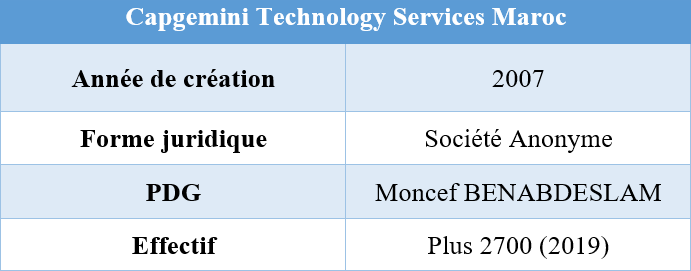
\includegraphics[width=0.8\textwidth]{latex_media/media/image4.png}
    \caption{Fiche d'identité de Capgemini Technology Services Maroc}
    \label{fig:fiche-capgemini-ts}
\end{figure}

\textbf{Capgemini Technology} Services Maroc est une entité spécialisée dans la fourniture de services technologiques et d'ingénierie. Depuis sa création, l'entreprise s'est imposée comme un partenaire incontournable pour de nombreuses organisations, grâce à son expertise et à son engagement envers l'innovation et la qualité des services.

\subsection{Organigramme de Capgemini TS Maroc}

Cette fiche présente l'organigramme de \textbf{Capgemini} TS Maroc, mettant en avant les rôles clés et les responsabilités au sein de notre structure. Elle illustre la hiérarchie et les interactions entre les différents départements, tout en soulignant l'importance de la collaboration pour atteindre nos objectifs.

\begin{figure}[htbp]
    \centering
    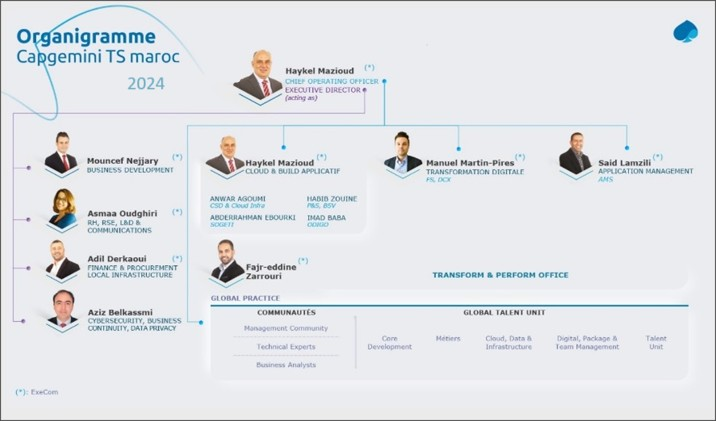
\includegraphics[width=0.9\textwidth]{latex_media/media/image5.jpeg}
    \caption{Organigramme de Capgemini TS Maroc}
    \label{fig:organigramme-capgemini}
\end{figure}

Chaque membre joue un rôle crucial dans le succès de nos projets, et cette représentation visuelle facilite la compréhension de notre organisation.

\subsection{Présentation du DigiCamp}

\begin{figure}[H]
\centering
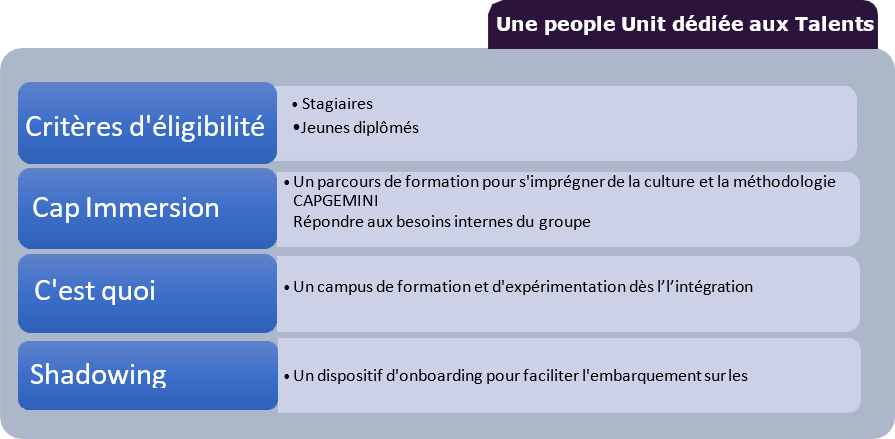
\includegraphics[width=0.8\textwidth]{latex_media/media/image6.png}
\caption{Plateforme Coding Challenge de Capgemini}
\label{fig:coding-challenge-capgemini}
\end{figure}

Dans un contexte où l'évaluation précise des compétences techniques des candidats est cruciale pour le recrutement efficace de talents, la plateforme Coding Challenge de \textbf{Capgemini} représente une réponse stratégique aux défis actuels. Cette plateforme innovante offre aux recruteurs un outil puissant pour évaluer objectivement les capacités des candidats à travers des tests techniques rigoureux. En automatisant une partie du processus de présélection, Coding Challenge permet non seulement de réduire les biais subjectifs associés aux méthodes traditionnelles, mais également d'accélérer significativement le temps nécessaire pour identifier les meilleurs talents. Cet outil s'inscrit dans une stratégie plus large visant à renforcer l'attrait de \textbf{Capgemini} en tant qu'employeur de choix, capable d'attirer et de retenir les profils les plus qualifiés dans le domaine de l'informatique.

DigiCamp a démarré en 2019 avec 39 collaborateurs qui travaillent sur 13 projets en utilisant diverses technologies. Le but est de permettre au talent de prendre son vol vers le staffing dans les projets en passant par les 3 principaux étapes :

\begin{itemize}
\item Cap Immersion.
\item Conditionnement en mode projet.
\item Formation L\&D et accompagnement dans les soft skills, technologies et méthodologie de travail.
\end{itemize}

Un portfolio ambitieux avec des technologies alignées aux besoins et contenant plus de 23 projets dont 15 applications en développement en 2020.

\section{Présentation du projet Quiz Agile}

\subsection{Contexte du projet}

Dans un environnement professionnel où l'agilité est devenue un facteur clé de succès, \textbf{Capgemini} a identifié le besoin de standardiser et d'optimiser l'évaluation des compétences de ses collaborateurs dans ce domaine. Ce besoin s'inscrit dans une stratégie plus large visant à renforcer la culture agile au sein de l'entreprise et à assurer l'excellence opérationnelle des équipes.

L'agilité, avec ses différentes méthodologies (Scrum, Kanban, SAFe, etc.), ses rôles spécifiques (Scrum Master, Product Owner) et ses pratiques (daily stand-up, sprint planning, retrospectives), représente un corpus de connaissances complexe dont la maîtrise est essentielle pour la réussite des projets informatiques modernes.

Jusqu'à présent, l'évaluation des compétences en agilité au sein de \textbf{Capgemini} reposait sur des approches variées et non standardisées : entretiens individuels, observations sur le terrain, ou questionnaires adhoc. Cette diversité d'approches rendait difficile la comparaison des niveaux de compétence entre équipes et limitait la capacité à identifier précisément les besoins de formation.

Par ailleurs, l'entreprise dispose déjà d'une plateforme de formation nommée NEXT, qui propose divers contenus pédagogiques mais ne dispose pas d'un module d'évaluation des compétences intégré. L'articulation entre évaluation et formation représente donc un enjeu majeur pour optimiser les parcours d'apprentissage.

\subsection{Problématique}

Dans le contexte spécifique de l'évaluation des compétences en agilité, le projet \textbf{QUIZ AGILE} vise à répondre à plusieurs problématiques interconnectées :

\begin{itemize}
\item \textbf{Comment standardiser l'évaluation des compétences en agilité à l'échelle de l'entreprise ?} L'absence d'un référentiel commun et d'outils standardisés rend difficile la comparaison des niveaux de compétence entre collaborateurs et entre équipes.
\item \textbf{Comment identifier avec précision les lacunes à combler ?} Les méthodes actuelles ne permettent pas toujours d'analyser finement les domaines spécifiques dans lesquels les collaborateurs ont besoin de renforcer leurs connaissances.
\item \textbf{Comment optimiser les parcours de formation en fonction des résultats d'évaluation ?} Sans lien direct entre évaluation et formation, il est difficile de proposer des parcours d'apprentissage véritablement personnalisés.
\end{itemize}


\begin{figure}[H]
\centering
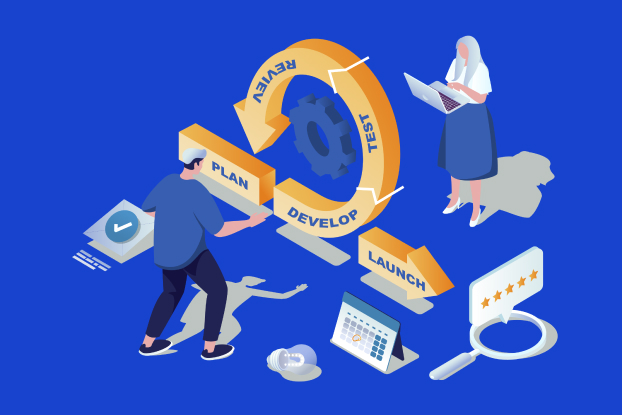
\includegraphics[width=0.8\textwidth]{latex_media/media/image7.jpeg}
\caption{Optimisation des parcours de formation selon les évaluations}
\label{fig:optimisation-parcours}
\end{figure}

\begin{itemize}
\item \textbf{Comment faciliter le suivi de l'évolution des compétences dans le temps ?} L'absence d'historisation des résultats limite la capacité à mesurer les progrès réalisés par les collaborateurs.
\end{itemize}

\subsection{Objectifs du projet}

Le projet \textbf{QUIZ AGILE} poursuit plusieurs objectifs stratégiques :

\begin{itemize}
\item \textbf{Standardiser l'évaluation des compétences en agilité} en proposant un référentiel commun et des outils d'évaluation uniformisés.
\item \textbf{Adapter la formation selon les besoins identifiés} grâce à une analyse précise des résultats et une intégration avec la plateforme de formation NEXT.
\item \textbf{Favoriser l'auto-apprentissage des collaborateurs} en leur permettant d'identifier leurs propres lacunes et de suivre leur progression.
\item \textbf{Fournir aux managers des tableaux de bord détaillés} sur les compétences de leurs équipes pour faciliter la prise de décision.
\item \textbf{Créer une base de connaissances évolutive} pouvant s'étendre à d'autres domaines de compétences au-delà de l'agilité.
\item \textbf{Préparer l'infrastructure pour une future intégration avec des fonctionnalités d'IA} qui permettront d'adapter dynamiquement les quiz en fonction des réponses précédentes.
\end{itemize}

\subsection{Population concernée}

Dans le contexte de la transformation digitale, le projet \textbf{QUIZ AGILE} s'adresse à un écosystème professionnel diversifié au sein de \textbf{Capgemini}, articulé autour de plusieurs catégories de professionnels stratégiques. Les collaborateurs techniques constituent le premier cercle de la population cible, comprenant :

\begin{itemize}
\item Les ingénieurs et développeurs impliqués dans les processus de développement logiciel
\item Les architectes systèmes et les experts en technologies émergentes
\item Les consultants spécialisés en transformation numérique
\end{itemize}

Les professionnels en management représentent un second périmètre crucial, intégrant :
\begin{itemize}
\item Les responsables d'unités opérationnelles
\item Les directeurs de projets technologiques
\item Les leaders en charge du développement organisationnel
\item Les responsables de pratiques métiers
\end{itemize}

L'écosystème de formation et de développement des compétences constitue un troisième groupe stratégique :
\begin{itemize}
\item Les formateurs spécialisés en méthodologies agiles
\item Les responsables du learning \& development
\item Les coaches certifiés en agilité
\item Les experts en gestion des compétences
\end{itemize}

\subsection{Solution proposée}

Face aux défis de l'évolution continue des compétences professionnelles, Quiz Agile émerge comme une solution technologique innovante d'évaluation et de développement des compétences en agilité.

La plateforme se caractérise par une approche méthodologique rigoureuse, articulée autour de plusieurs axes stratégiques :

\subsubsection{Évaluation standardisée des compétences}

Quiz Agile propose un dispositif d'évaluation scientifique et objectif, reposant sur :
\begin{itemize}
\item Des questionnaires à choix multiples hautement paramétrables
\item Un référentiel de compétences normalisé
\item Une approche d'évaluation multicritères
\end{itemize}

\subsubsection{Architecture fonctionnelle innovante}

La solution intègre des fonctionnalités technologiquement avancées :
\begin{itemize}
\item Création de quiz par des experts métiers
\item Passation de tests en environnement numérique sécurisé
\item Analyse approfondie et contextualisation des résultats
\item Recommandations de parcours de formation personnalisés
\item Tableaux de bord décisionnels pour les managers
\end{itemize}

\subsubsection{Intégration technologique et écosystémique}

Quiz Agile se distingue par sa capacité d'intégration :
\begin{itemize}
\item Interconnexion native avec la plateforme de formation NEXT
\item Mécanisme d'authentification unique sécurisé
\item Synchronisation dynamique des données
\item Compatibilité multiplateforme et multiappareils
\end{itemize}

\subsubsection{Bénéfices organisationnels stratégiques}

Quiz Agile vise à générer une valeur ajoutée significative :
\begin{itemize}
\item Identification précise et objective des compétences
\item Personnalisation des trajectoires de développement professionnel
\item Optimisation des investissements en formation
\item Accélération de la transformation culturelle et méthodologique
\end{itemize}

\subsection{Conduite et planification du projet}

La planification est cruciale pour le succès du projet. Elle commence par la conception, où les objectifs et les besoins des utilisateurs sont identifiés. Ensuite, le cadrage fonctionnel et technique établit les fonctionnalités requises et les technologies à utiliser. La phase de codage suit, durant laquelle les développeurs créent le produit selon les spécifications. Ensuite, des tests internes sont effectués pour détecter et corriger les erreurs. Une fois ces tests complétés, le produit est soumis à une validation avec le client pour s'assurer qu'il répond aux attentes. Cette approche structurée garantit un développement efficace et réduit les risques de dérives.

\subsubsection{Intégration et formation continue}

Lors de mon intégration chez \textbf{Capgemini}, j'ai rejoint l'équipe de développement du projet Quiz Agile en tant que Software Engineer Intern. Cette expérience m'a permis de participer activement aux différentes phases de développement de l'application, qui repose sur un écosystème technologique moderne.

Parallèlement, j'ai suivi des formations ciblées sur ces technologies via :
\begin{itemize}
\item La plateforme NEXT de \textbf{Capgemini}
\item La plateforme Udemy
\item Des sessions de formation internes
\end{itemize}

J'ai également complété des formations obligatoires sur :
\begin{itemize}
\item L'éthique professionnelle
\item Le code de conduite de \textbf{Capgemini}
\item La sécurité informatique
\item Les politiques de propriété intellectuelle
\end{itemize}

\subsection{Méthodologie du travail : Agile \& Scrum}

Le projet \textbf{Quiz Agile} a été développé en suivant rigoureusement la méthodologie Agile Scrum, permettant :
\begin{itemize}
\item Un développement itératif et incrémental
\item Une adaptation continue aux besoins
\item Une livraison rapide de valeur métier
\end{itemize}

Les réunions quotidiennes (Daily Scrum) jouent un rôle central dans cette méthodologie, favorisant la communication et la coordination de l'équipe.

\begin{figure}[H]
\centering
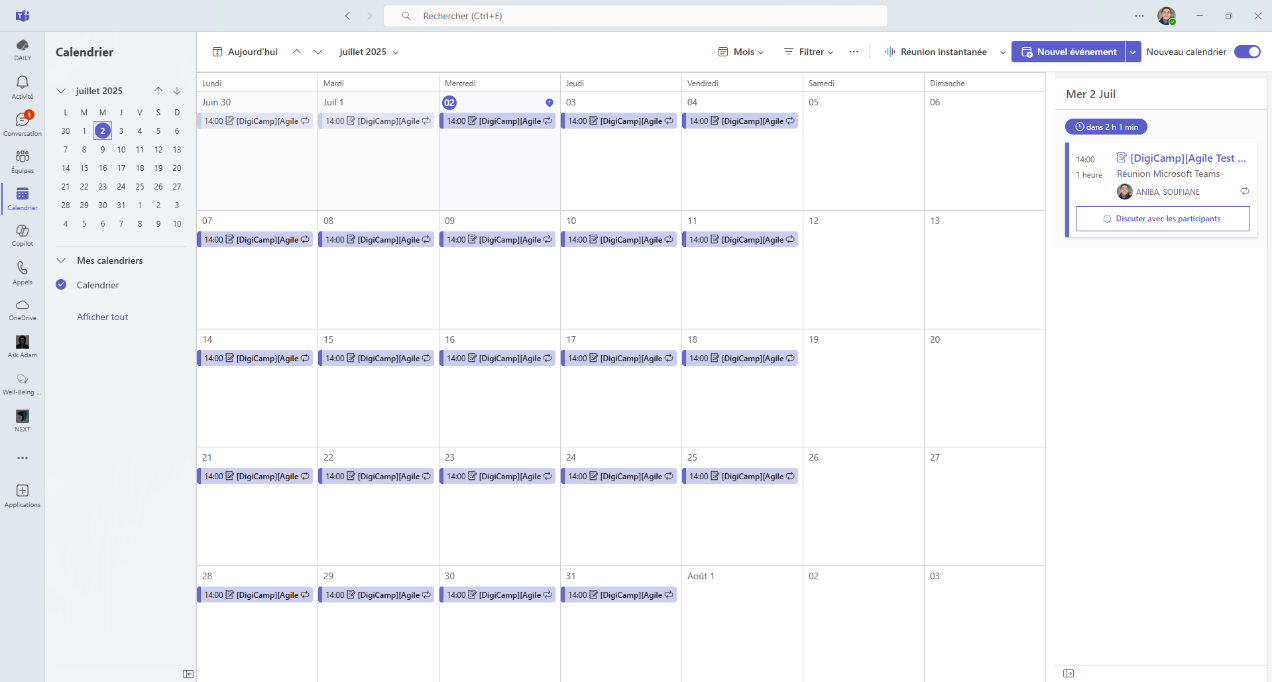
\includegraphics[width=0.8\textwidth]{latex_media/media/image9.png}
\caption{Organisation des réunions quotidiennes (Daily Scrum)}
\label{fig:daily-scrum}
\end{figure}

Ces réunions quotidiennes de synchronisation permettent à l'équipe de partager les avancées, identifier les blocages et coordonner les efforts pour atteindre les objectifs du sprint.

\cleardoublepage
\section{Conclusion}

Ce premier chapitre a permis de dresser un panorama de \textbf{Capgemini}, de ses activités et de ses engagements, tout en soulignant le rôle central de l'innovation dans ses projets de transformation numérique.

L'analyse du contexte a mis en évidence les limites des processus actuels d'évaluation des compétences en agilité : lenteur, subjectivité, difficulté de standardisation et manque d'outils d'analyse. Ces constats révèlent la nécessité de disposer d'une solution plus rapide, objective et accessible.

Le projet \textbf{QUIZ AGILE} s'inscrit dans cette perspective en proposant une application web intégrée utilisant des technologies modernes. Cette solution vise à améliorer l'évaluation des compétences, faciliter l'adaptation des formations et fournir des outils d'analyse performants, tout en offrant une alternative innovante et efficace aux processus traditionnels.

% ============================================
% CHAPITRE 2 - Analyse et Spécification des besoins
% ============================================

\cleardoublepage
\thispagestyle{empty}
\begin{center}
    \vspace*{4cm}
    {\Huge \textbf{Chapitre 2}}\\[1.5cm]
    {\LARGE \textbf{Analyse et Spécification des besoins}}
\end{center}
\cleardoublepage

\refstepcounter{chapter}
\addcontentsline{toc}{chapter}{Chapitre \thechapter: Analyse et Spécification des besoins}
\markboth{Chapitre \thechapter: Analyse et Spécification des besoins}{}
\setcounter{section}{0}

\section{Introduction}

La phase de conception et de modélisation constitue une étape cruciale
dans le cycle de développement du projet Quiz Agile. Elle permet de
traduire les besoins identifiés lors de l'analyse
préliminaire en une architecture technique et fonctionnelle cohérente.
Ce chapitre présente de manière détaillée l'ensemble des
travaux de conception réalisés, depuis l'analyse des
besoins jusqu'aux choix d'architecture
technique. Nous y aborderons successivement l'analyse
des exigences fonctionnelles et non fonctionnelles,
l'identification des acteurs du système, la modélisation
conceptuelle à travers différents diagrammes UML, et enfin les choix
techniques qui ont guidé l'implémentation du projet.
Cette démarche méthodique vise à garantir que le système final réponde
parfaitement aux attentes des utilisateurs tout en
s'inscrivant dans une architecture évolutive et
maintenable.

\section{Exigences fonctionnelles}

Les exigences fonctionnelles du projet Quiz Agile ont été établies à partir des besoins exprimés par les parties prenantes et des objectifs stratégiques de l'entreprise. Ces exigences définissent les fonctionnalités que le système doit offrir pour répondre aux attentes des utilisateurs.

\subsection{Gestion des utilisateurs}

\begin{itemize}
\item Authentification des utilisateurs avec différents rôles (Administrateur, Coach, Collaborateur)
\item Gestion des profils utilisateurs (création, modification, suppression)
\item Attribution et gestion des droits d'accès selon les rôles
\end{itemize}

\subsection{Gestion des quiz}

\begin{itemize}
\item Création de quiz par les coachs avec titre, description et paramètres
\item Configuration des quiz (durée, nombre de tentatives autorisées, seuil de réussite)
\item Importation et exportation de questions au format standardisé
\item Catégorisation des quiz par thématique et niveau de difficulté
\item Génération d'URL de partage pour diffusion aux collaborateurs
\end{itemize}

\subsection{Gestion des questions}

\begin{itemize}
\item Création de questions de différents types (QCM, vrai/faux, réponses multiples)
\item Association d'options de réponse avec indication des réponses correctes
\item Attribution d'un niveau de difficulté et de mots-clés aux questions
\item Réutilisation des questions dans différents quiz
\item Suggestion intelligente de questions basée sur l'historique et les thématiques
\end{itemize}

\subsection{Passage des quiz}

\begin{itemize}
\item Interface intuitive pour répondre aux questions
\item Chronomètre pour respecter la durée impartie
\item Navigation entre les questions
\item Possibilité de marquer des questions pour y revenir plus tard
\end{itemize}

\subsection{Évaluation et résultats}

\begin{itemize}
\item Calcul automatique des scores
\item Affichage des réponses correctes et des explications après soumission
\item Génération de rapports détaillés pour les participants
\item Attribution de badges et récompenses selon les performances
\item Historique des tentatives et progression dans le temps
\end{itemize}

\subsection{Analyse et reporting}

\begin{itemize}
\item Tableau de bord pour les coachs avec statistiques globales
\item Analyse des performances par équipe, thématique ou question
\item Identification des points forts et des axes d'amélioration
\item Exportation des résultats pour analyse externe
\item Recommandations personnalisées de formation
\end{itemize}

\subsection{Intégration avec la plateforme NEXT}

\begin{itemize}
\item Authentification unique (SSO) entre Quiz Agile et NEXT
\item Synchronisation des données utilisateurs
\item Intégration des quiz dans les parcours de formation NEXT
\item Partage des résultats avec la plateforme NEXT
\end{itemize}

\section{Spécifications Non Fonctionnelles}

Les exigences non fonctionnelles définissent les critères de qualité et les contraintes techniques que le système doit respecter.

\subsection{Performance}

\begin{itemize}
\item Temps de réponse inférieur à 2 secondes pour les opérations courantes
\item Capacité à gérer simultanément jusqu'à 200 utilisateurs actifs
\item Optimisation des requêtes de base de données pour minimiser la latence
\item Mise en cache des données fréquemment accédées
\end{itemize}

\subsection{Sécurité}

\begin{itemize}
\item Protection des données personnelles conformément au RGPD
\item Authentification sécurisée avec support de l'authentification à deux facteurs
\item Chiffrement des données sensibles en transit et au repos
\item Journalisation des actions critiques pour audit
\item Protection contre les attaques courantes (injection SQL, XSS, CSRF)
\end{itemize}

\subsection{Disponibilité et fiabilité}

\begin{itemize}
\item Disponibilité du système 99,9\% du temps (hors maintenance planifiée)
\item Sauvegarde quotidienne des données avec rétention de 30 jours
\item Plan de reprise d'activité avec un RTO (Recovery Time Objective) de 4 heures
\item Mécanismes de détection et de notification des erreurs
\end{itemize}

\subsection{Maintenabilité}

\begin{itemize}
\item Architecture modulaire facilitant l'évolution du système
\item Documentation complète du code et de l'architecture
\item Tests automatisés couvrant au moins 80\% du code
\item Respect des standards de codage et des bonnes pratiques
\end{itemize}

\subsection{Scalabilité}

\begin{itemize}
\item Architecture permettant une montée en charge horizontale
\item Conception adaptée à une future migration vers les microservices
\item Séparation claire des responsabilités pour faciliter la distribution
\end{itemize}

\subsection{Utilisabilité}

\begin{itemize}
\item Interface utilisateur intuitive et responsive
\item Support multilingue (français et anglais dans un premier temps)
\item Accessibilité conforme aux normes WCAG 2.1 niveau AA
\item Compatibilité avec les principaux navigateurs (Chrome, Firefox, Safari, Edge)
\item Support des appareils mobiles et tablettes
\end{itemize}

\subsection{Interopérabilité}

\begin{itemize}
\item API RESTful documentée pour l'intégration avec des systèmes tiers
\item Support des formats d'échange standards (JSON, XML)
\end{itemize}

\section{Analyse des Acteurs et des Cas d'Utilisation}

L'identification des acteurs et de leurs rôles est une étape cruciale dans la conception d'une application. Elle permet de comprendre les besoins spécifiques de chaque utilisateur et de créer une expérience utilisateur optimale. En définissant clairement les rôles et les fonctionnalités associées à chaque type d'utilisateur, on peut garantir que l'application répond aux attentes de chacun et facilite les interactions entre les différents acteurs.

\subsection{Identification des acteurs}

Un acteur est l'idéalisation d'un rôle joué par une personne, un matériel ou un logiciel qui interagit directement avec le système en question. Il peut consulter et / ou modifier directement l'état du système en émettant ou recevant des messages susceptibles d'être porteurs de données.

\begin{figure}[H]
\centering
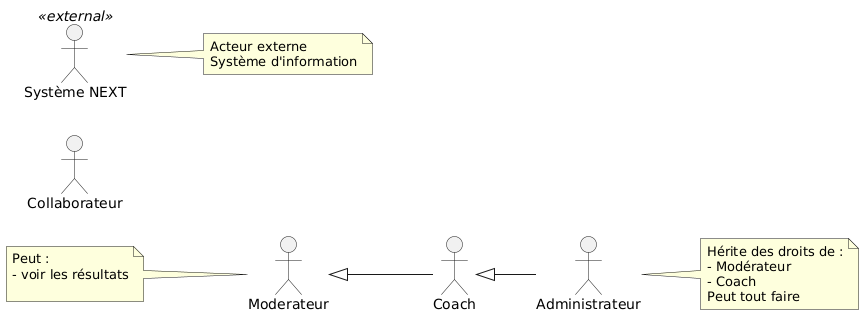
\includegraphics[width=0.9\textwidth]{latex_media/media/image13.png}
\caption{Acteurs principaux du système Quiz Agile}
\label{fig:acteurs-principaux}
\end{figure}

Dans le cadre du projet QUIZ AGILE, plusieurs acteurs clés interagissent avec l'application mobile et la plateforme web. Voici une description de chacun d'eux :

\subsubsection{Administrateur}

\begin{itemize}
\item Responsable de la configuration globale du système
\item Gère les utilisateurs et leurs droits
\item Supervise l'ensemble des activités sur la plateforme
\item Accède aux statistiques globales et aux journaux d'audit
\end{itemize}

\subsubsection{Coach}

\begin{itemize}
\item Crée et gère les quiz et les questions
\item Configure les paramètres des évaluations
\item Analyse les résultats des collaborateurs
\item Identifie les besoins en formation
\item Génère des rapports d'analyse
\end{itemize}

\subsubsection{Collaborateur}

\begin{itemize}
\item Passe les quiz d'évaluation
\item Consulte ses résultats et son historique
\item Suit sa progression dans le temps
\item Reçoit des recommandations personnalisées
\end{itemize}

\subsubsection{Système NEXT}

\begin{itemize}
\item Échange des données avec Quiz Agile
\item Authentifie les utilisateurs via SSO
\item Intègre les quiz dans les parcours de formation
\item Récupère les résultats des évaluations
\end{itemize}

\subsection{Diagramme de Cas d'Utilisation}

Le diagramme de cas d'utilisation est un outil d'analyse puissant qui permet de visualiser les différents cas d'utilisation de l'application et les fonctionnalités associées aux interactions avec les acteurs, offrant ainsi une compréhension globale des besoins des utilisateurs et des objectifs du système.

\begin{figure}[htbp]
    \centering
    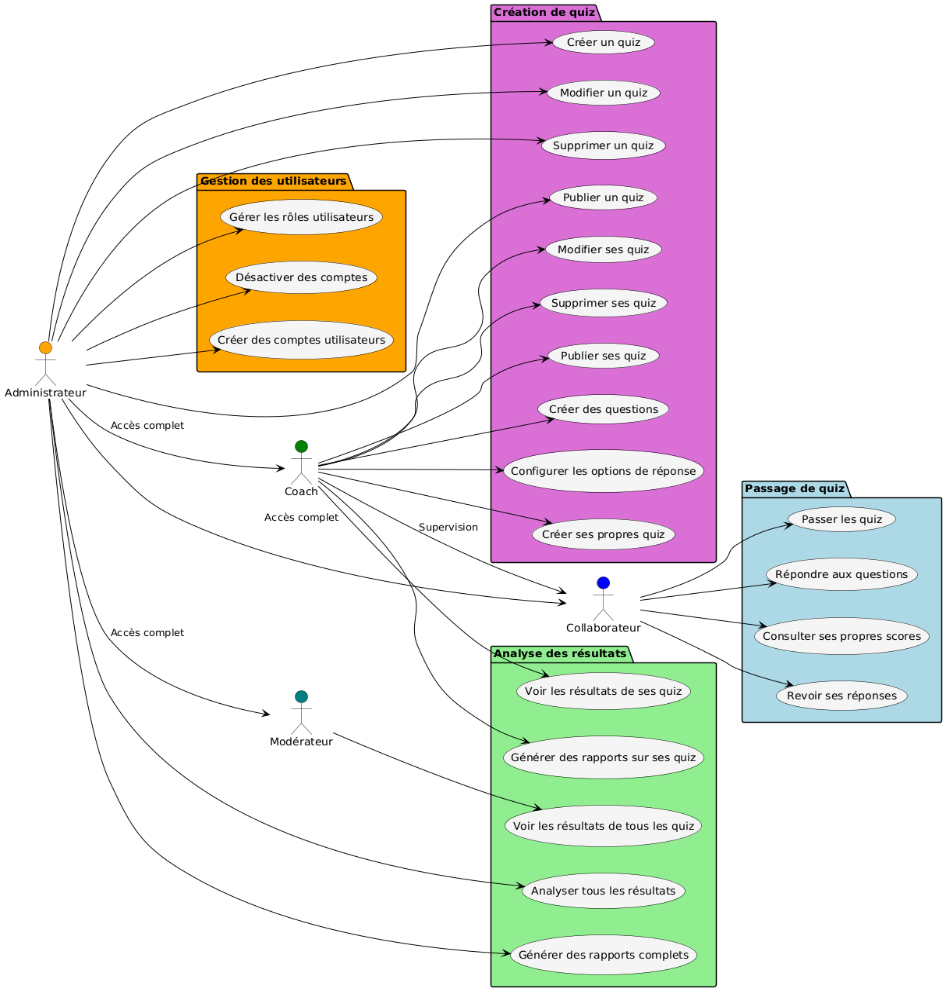
\includegraphics[width=0.7\textwidth]{latex_media/media/image14.png}
    \caption{Diagramme de cas d'utilisation du système Quiz Agile}
    \label{fig:cas-utilisation}
\end{figure}

Le diagramme de cas d'utilisation ci-dessus illustre les principales interactions entre les acteurs et le système Quiz Agile. Le diagramme met en évidence les actions principales accessibles aux différents acteurs après authentification. Cette modélisation permet de comprendre les interactions et les périmètres de responsabilité au sein de l'application Quiz Agile.

\section{Conclusion}

Ce chapitre a présenté l'analyse détaillée des besoins fonctionnels et non-fonctionnels du projet Quiz Agile. L'identification claire des acteurs et de leurs rôles, ainsi que la modélisation des cas d'utilisation, fournissent une base solide pour la conception et le développement du système. Cette approche méthodique garantit que la solution finale répondra aux attentes de tous les utilisateurs tout en respectant les contraintes techniques et de qualité requises.

% ============================================
% CHAPITRE 3 - Conception et Mise en place du système
% ============================================

\cleardoublepage
\thispagestyle{empty}
\begin{center}
    \vspace*{4cm}
    {\Huge \textbf{Chapitre 3}}\\[1.5cm]
    {\LARGE \textbf{Conception et Mise en place du système}}
\end{center}
\cleardoublepage

\refstepcounter{chapter}
\addcontentsline{toc}{chapter}{Chapitre \thechapter: Conception et Mise en place du système}
\markboth{Chapitre \thechapter: Conception et Mise en place du système}{}
\setcounter{section}{0}

\section{Introduction}

La conception constitue une étape clé entre la spécification des besoins et l'implémentation. Elle permet de représenter, sous forme de modèles, la structure et le comportement du système afin de garantir sa cohérence, sa robustesse et sa maintenabilité.

Dans le cadre du projet \textbf{QUIZ AGILE}, la conception se décline en deux volets complémentaires :
\begin{itemize}
    \item la \textbf{modélisation dynamique} décrivant les comportements, scénarios et flux de données (diagrammes de séquence et d'activités)
    \item la \textbf{modélisation statique} mettant en avant la structure du système (diagramme de classes et modèle relationnel) ainsi que l'architecture logicielle de déploiement
\end{itemize}

\section{Architecture du système}

\begin{figure}[htbp]
    \centering
    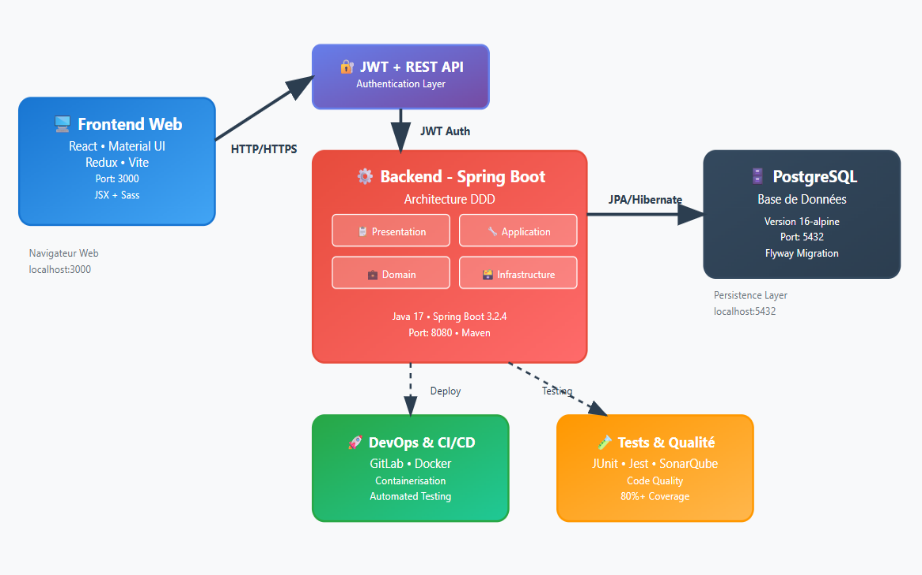
\includegraphics[width=0.9\textwidth]{latex_media/media/Architecture_globale.png}
    \caption{Architecture globale du système Quiz Agile}
    \label{fig:architecture-globale}
\end{figure}

L'architecture globale du système Quiz Agile illustre l'organisation complète des composants techniques, depuis l'interface utilisateur frontend jusqu'à la base de données, en passant par la couche d'authentification, les services backend et les outils de déploiement et de test.

\subsection{Architecture logicielle}

L'architecture logicielle du système Quiz Agile repose sur une approche en couches (layered architecture) qui garantit une séparation claire des responsabilités et facilite la maintenance et l'évolutivité du système.

\subsubsection{Architecture 3-tiers}

Le système adopte une architecture 3-tiers classique :

\begin{itemize}
    \item \textbf{Couche Présentation} : Interface utilisateur développée en React
    \item \textbf{Couche Métier} : Logique applicative implémentée avec Spring Boot
    \item \textbf{Couche Données} : Base de données relationnelle MySQL
\end{itemize}

\subsubsection{Patron d'architecture MVC}

L'application respecte le patron Modèle-Vue-Contrôleur (MVC) :

\begin{itemize}
    \item \textbf{Modèle} : Entités JPA et services métier
    \item \textbf{Vue} : Composants React pour l'interface utilisateur
    \item \textbf{Contrôleur} : REST Controllers Spring Boot
\end{itemize}

\subsection{Architecture de déploiement}

L'architecture de déploiement prévoit une séparation entre l'environnement de développement et l'environnement de production, avec des mécanismes de CI/CD pour automatiser les déploiements.

\section{Modélisation UML}

La modélisation UML (Unified Modeling Language) constitue une étape essentielle de la conception du système Quiz Agile. Elle permet de représenter visuellement la structure, le comportement et les interactions du système à travers différents types de diagrammes.

\subsection{Diagramme de classes}

Le diagramme de classes représente la structure statique du système en montrant les classes, leurs attributs, leurs méthodes et les relations entre elles. Cette modélisation UML offre une compréhension approfondie de la structure interne du code et de ses interactions complexes.

\begin{figure}[H]
\centering
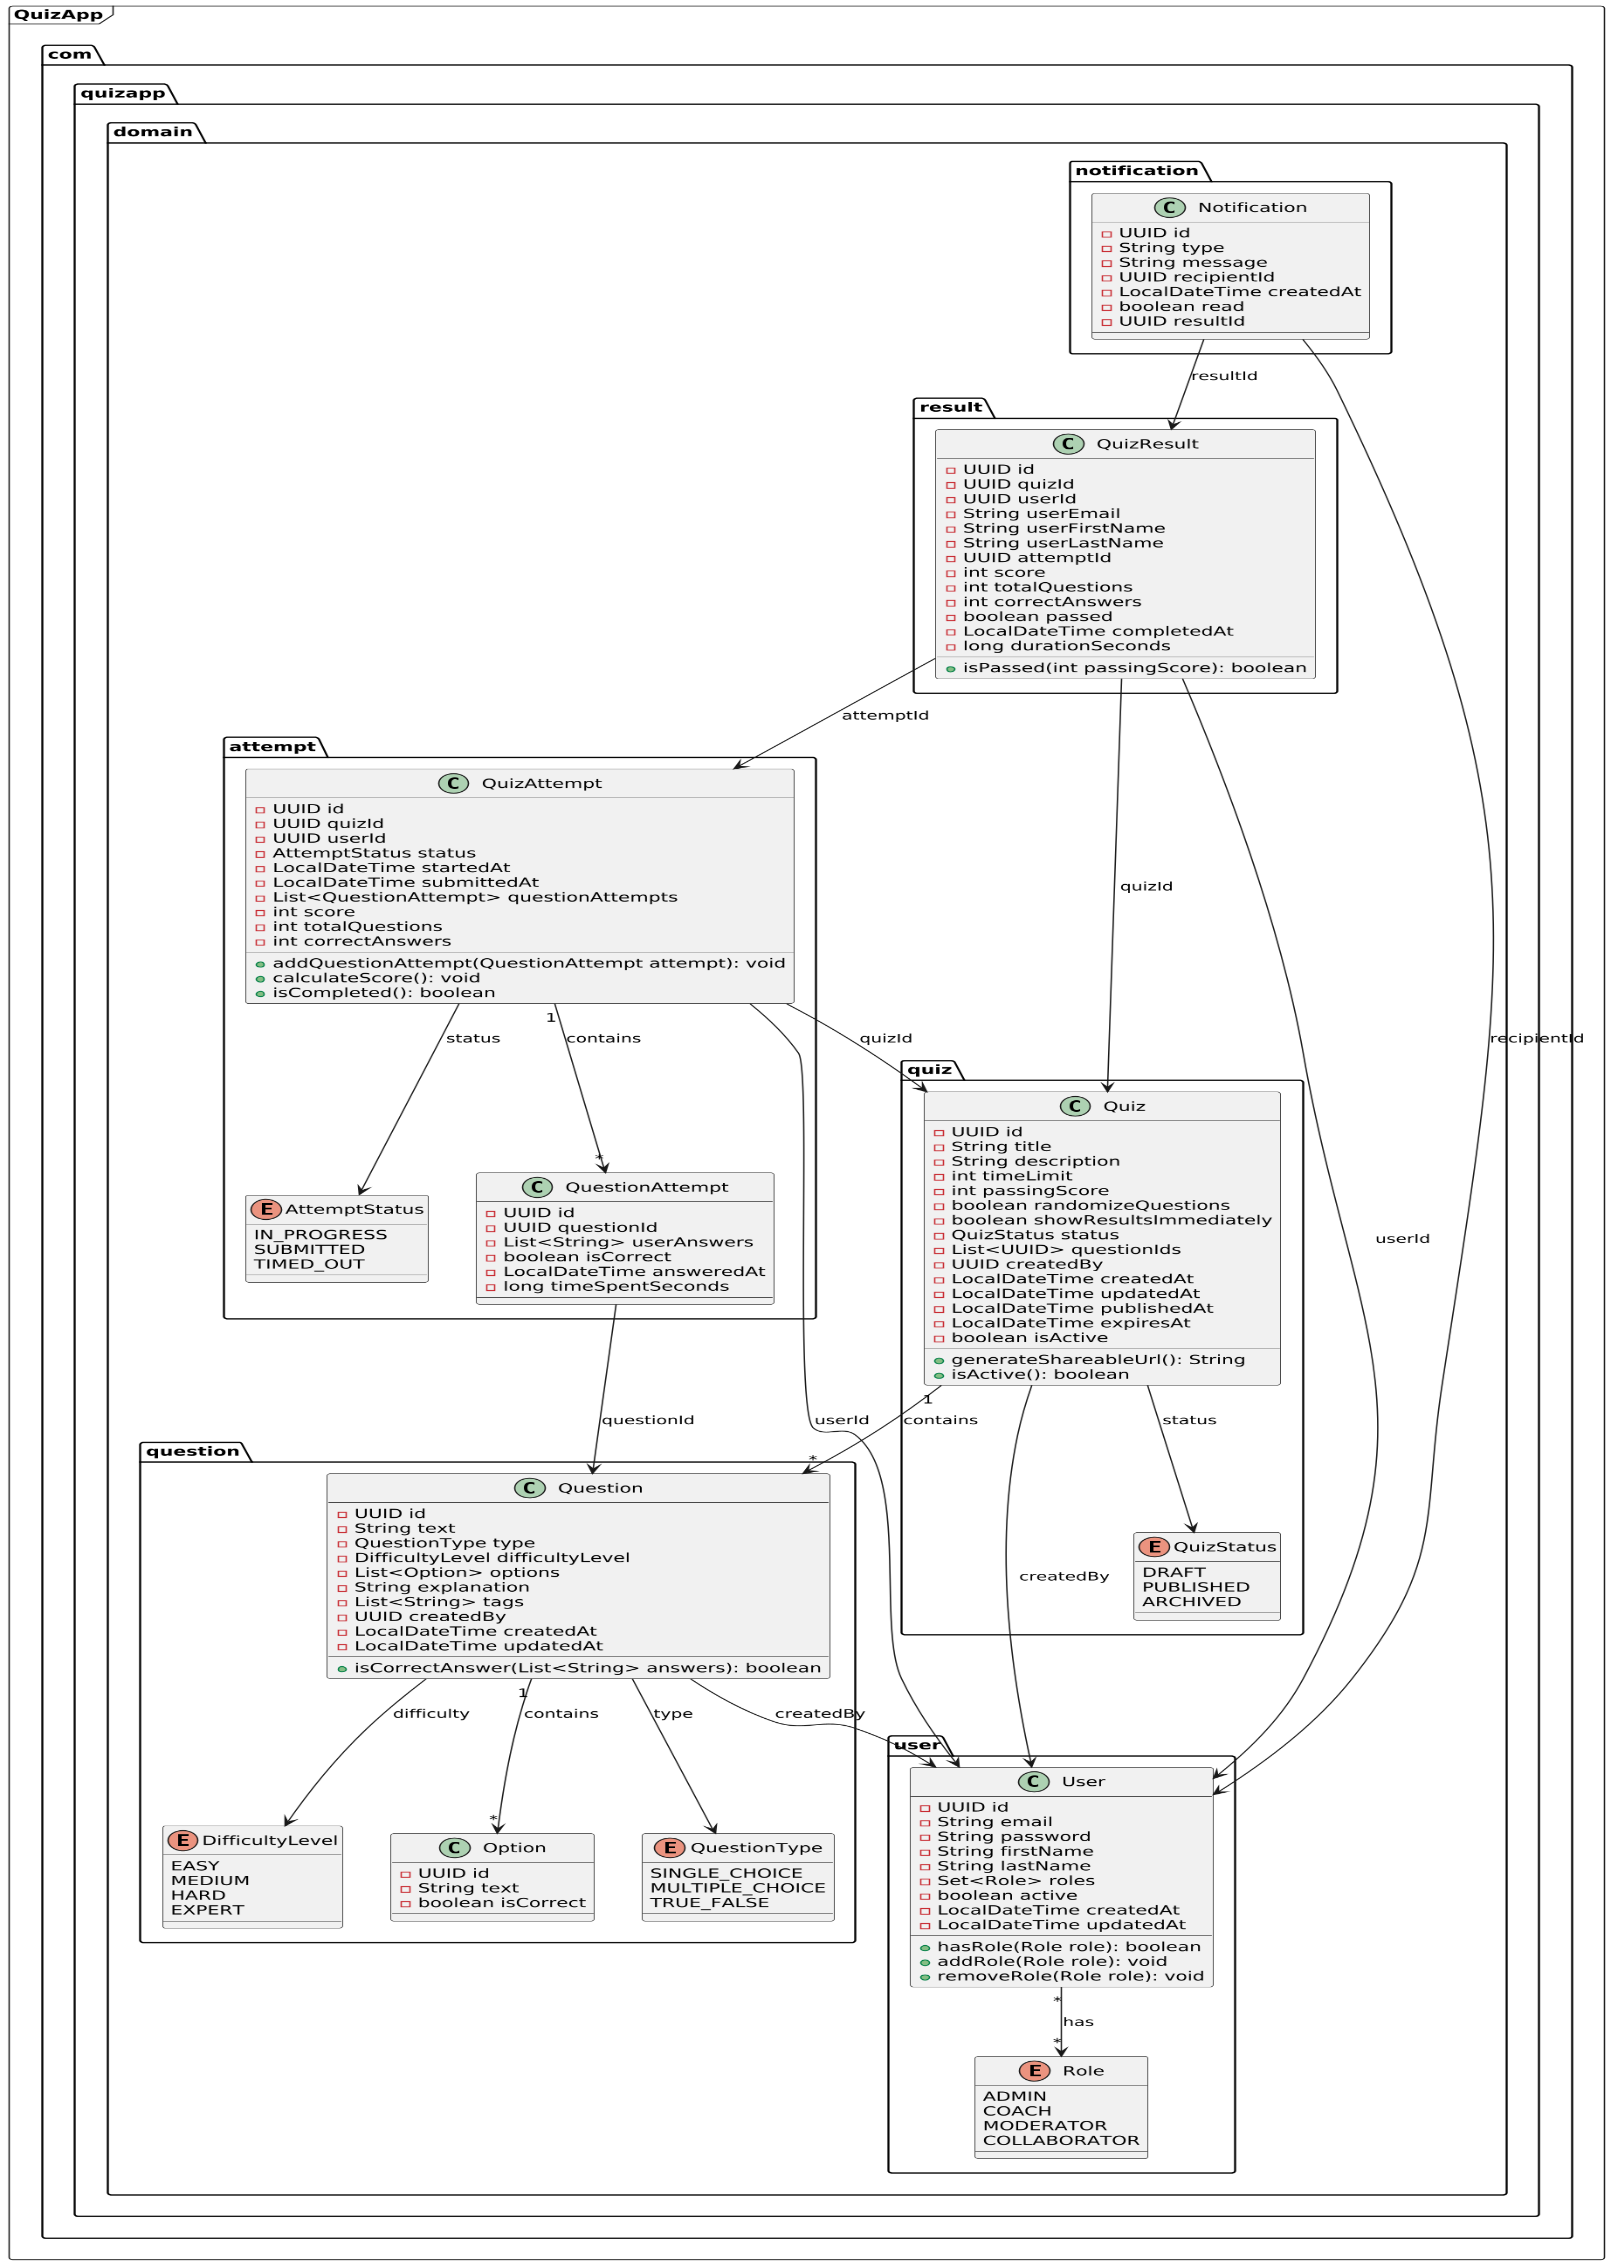
\includegraphics[width=0.9\textwidth]{latex_media/media/image16.png}
\caption{Diagramme de classes du système Quiz Agile}
\label{fig:diagramme-classes}
\end{figure}

Le diagramme représente un système de quiz en ligne avec 6 packages principaux organisés dans le cadre "Agile Quiz" :

\begin{enumerate}
\item \textbf{Model} : Contient les entités principales (User, Quiz, Question, QuizAttempt)
\item \textbf{Repository} : Interfaces d'accès aux données utilisant Spring Data JPA
\item \textbf{Service} : Logique métier et traitements des données
\item \textbf{Controller} : Endpoints REST pour l'API
\item \textbf{DTO} : Objets de transfert de données pour les échanges API
\item \textbf{Config} : Configuration de sécurité et JWT
\end{enumerate}

\subsection{Diagramme de paquetages}

Le diagramme de paquetages offre une vue d'ensemble de l'organisation structurelle du système Quiz Agile. Il présente les différents modules et leurs relations, facilitant la compréhension de l'architecture globale.

\begin{figure}[H]
\centering
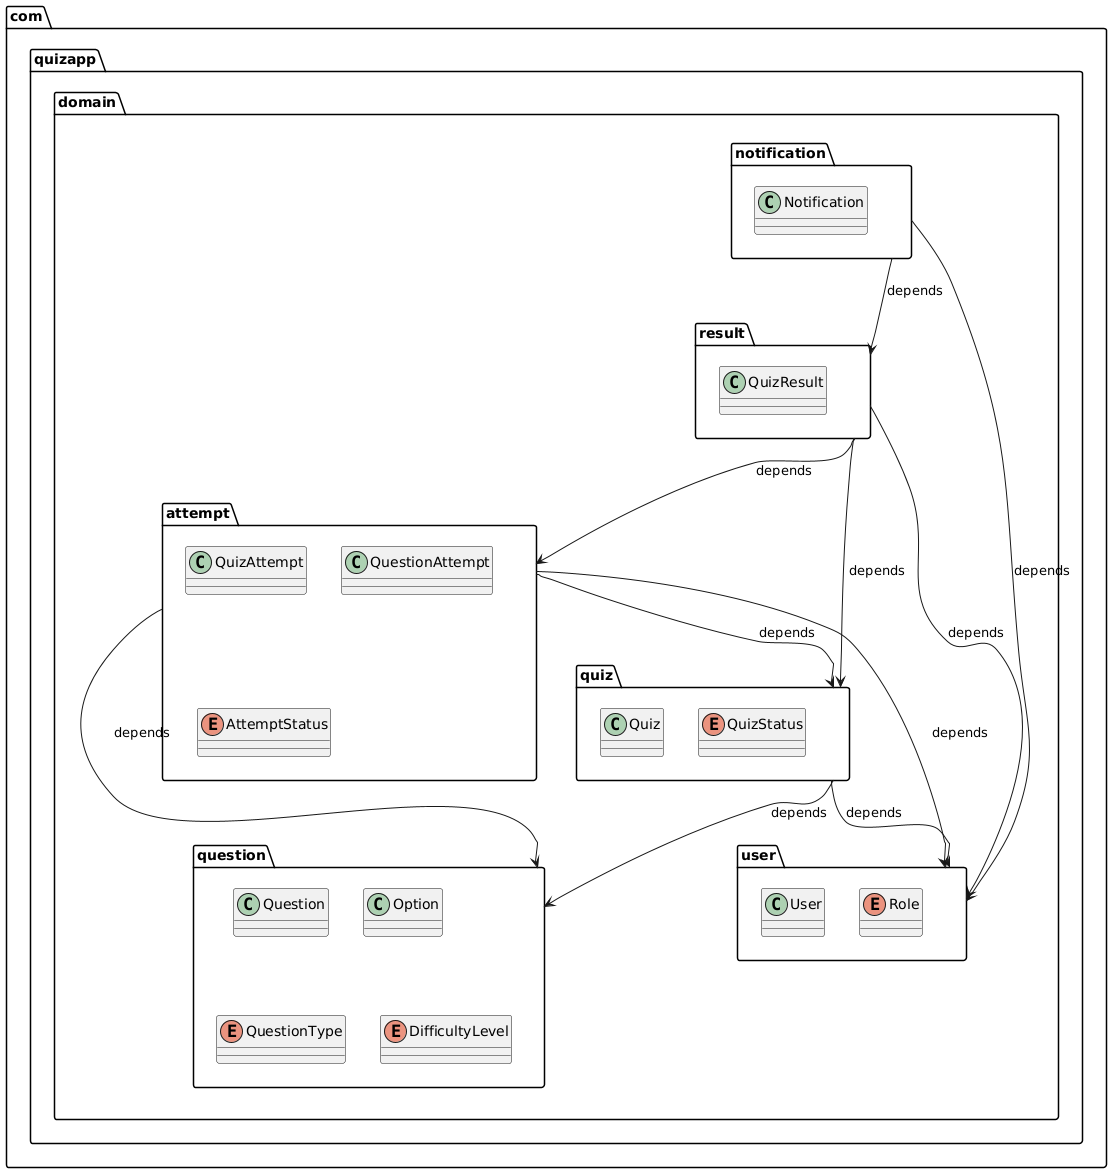
\includegraphics[width=0.9\textwidth]{latex_media/media/image17.png}
\caption{Diagramme de paquetages de l'architecture système}
\label{fig:diagramme-paquetages}
\end{figure}

Cette représentation modulaire favorise une approche de développement claire et maintient une séparation logique entre les différentes responsabilités du système.

\subsection{Diagramme de séquence}

Le diagramme de séquence est un diagramme d'interaction qui détaille le déroulement temporel des échanges entre les différents objets du système. Il représente la chronologie des appels de méthodes et des interactions pour un scénario d'usage particulier.

\begin{figure}[H]
\centering
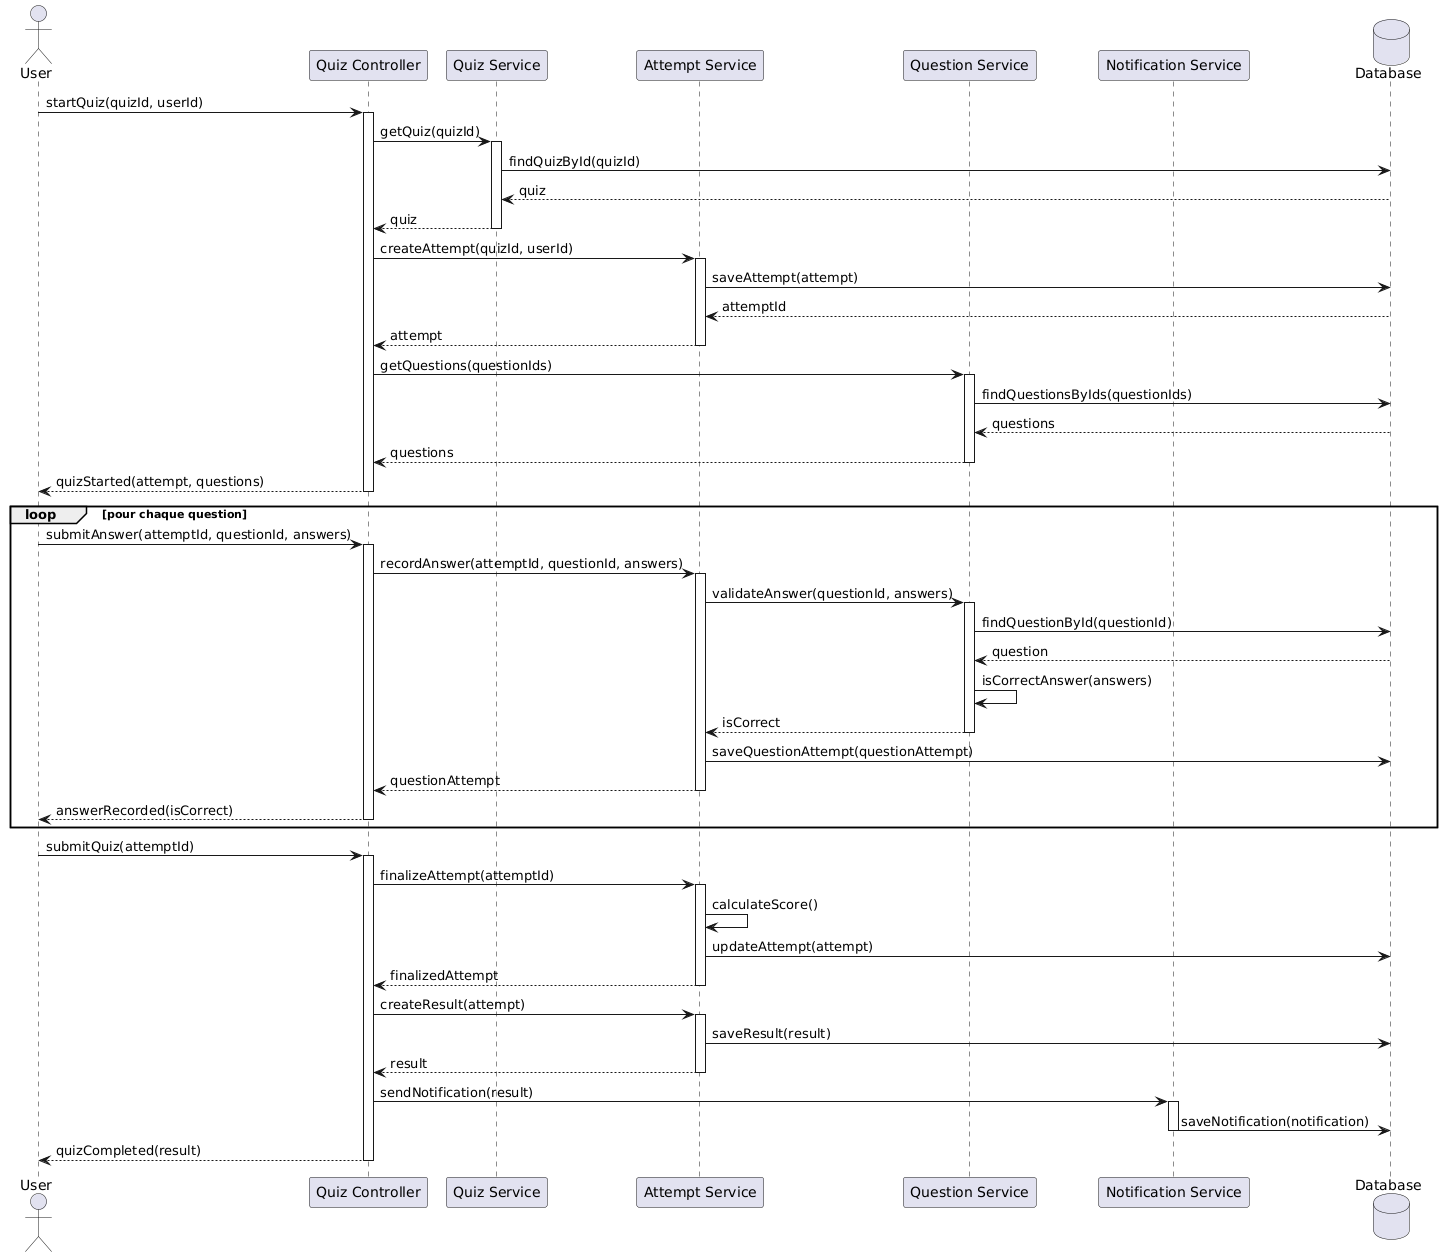
\includegraphics[width=0.9\textwidth]{latex_media/media/image19.png}
\caption{Diagramme de séquence du système Quiz Agile}
\label{fig:diagramme-sequence}
\end{figure}

Ce diagramme illustre les interactions principales lors du processus de création et de passage d'un quiz, mettant en évidence la communication entre les couches de l'architecture.

\subsubsection{Diagramme de séquence - Flux de création et export de quiz}

Ce diagramme de séquence détaillé illustre spécifiquement le flux de création d'un quiz et le processus d'export PDF, mettant en évidence les différents composants de notre solution fondée sur l'architecture hexagonale.

\begin{figure}[H]
\centering
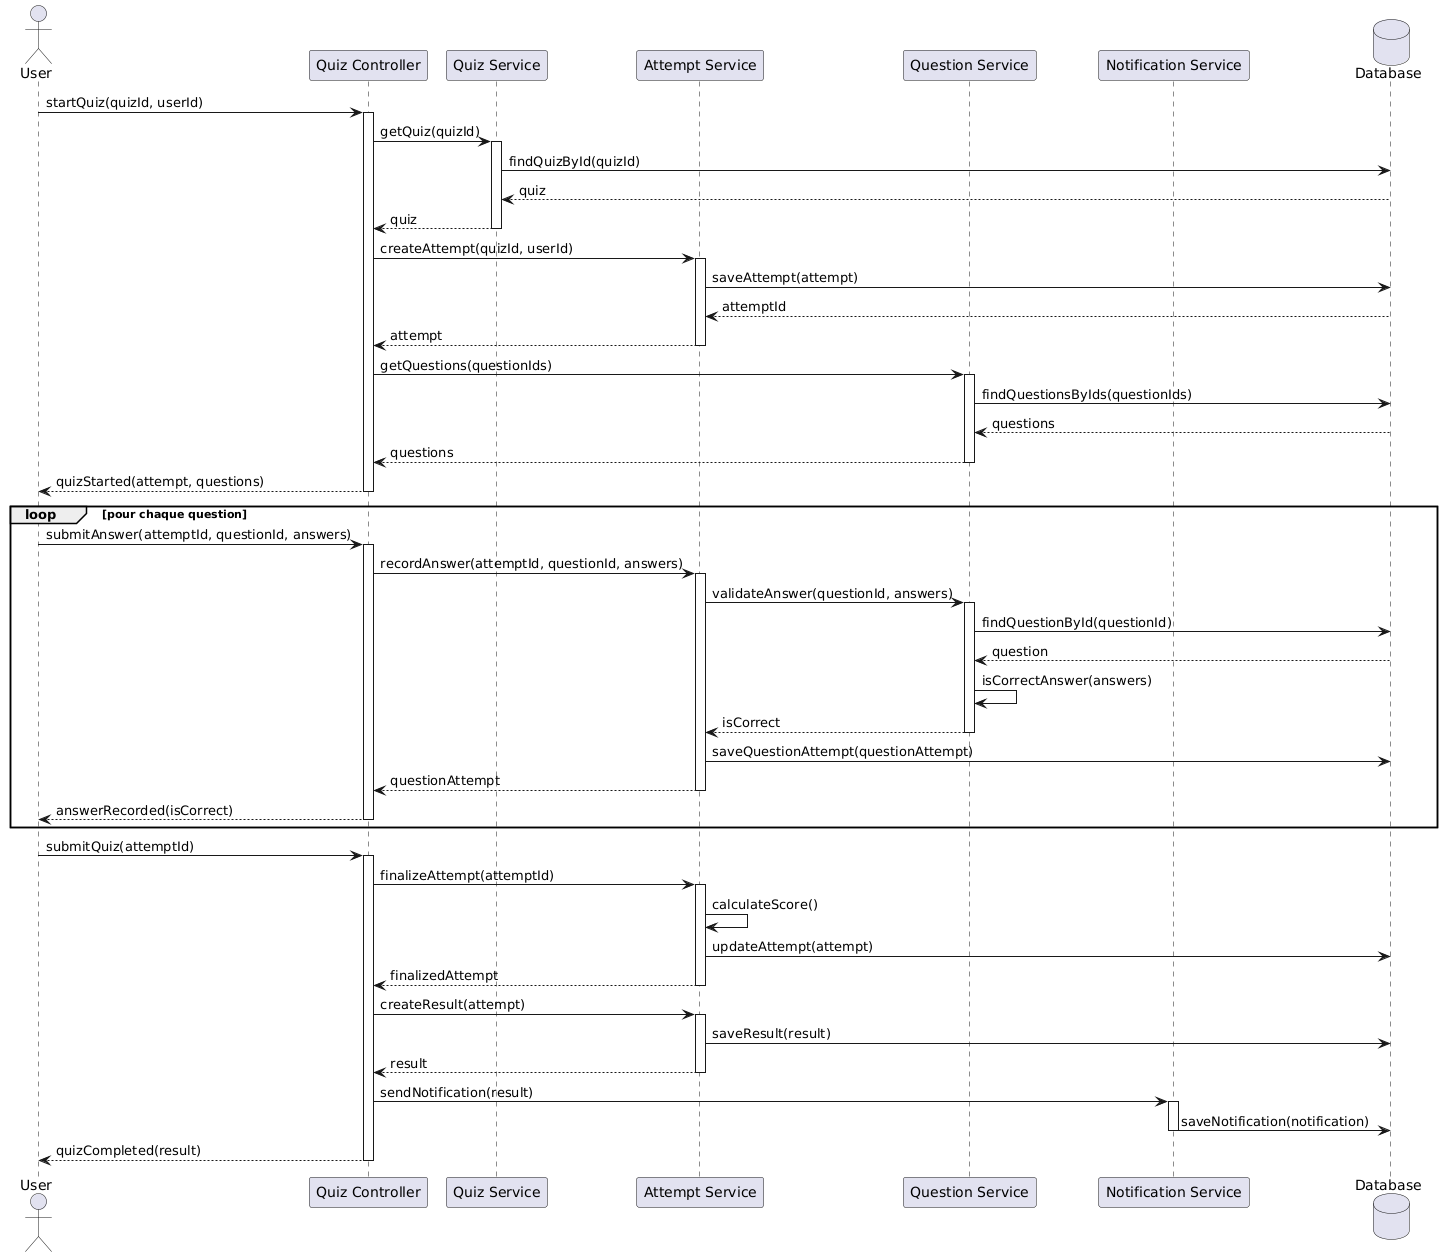
\includegraphics[width=1.0\textwidth]{latex_media/media/sequence_diagram_quiz_creation.png}
\caption{Diagramme de séquence - Flux de création de quiz et export PDF}
\label{fig:sequence-creation-quiz}
\end{figure}

Ce diagramme montre les interactions entre :
\begin{itemize}
\item \textbf{React Frontend} : Interface utilisateur pour la création de quiz
\item \textbf{QuizController} : Point d'entrée REST pour les requêtes de création
\item \textbf{QuizService} : Logique métier pour la gestion des quiz
\item \textbf{QuizMapper} : Conversion entre entités et DTOs
\item \textbf{Quiz Entity} : Modèle de données principal
\item \textbf{QuizRepository} : Accès aux données PostgreSQL
\item \textbf{PdfExportService} : Service d'export en format PDF
\end{itemize}

Le flux illustre les étapes depuis la soumission d'un nouveau quiz jusqu'à la génération du fichier PDF de résultats, démontrant la séparation claire des responsabilités dans notre architecture hexagonale.

\subsection{Diagramme d'activité}

Le diagramme d'activité représente le flux de processus et les décisions dans le système. Il modélise les activités, les transitions et les points de décision pour illustrer le comportement dynamique du système.

\begin{figure}[htbp]
    \centering
    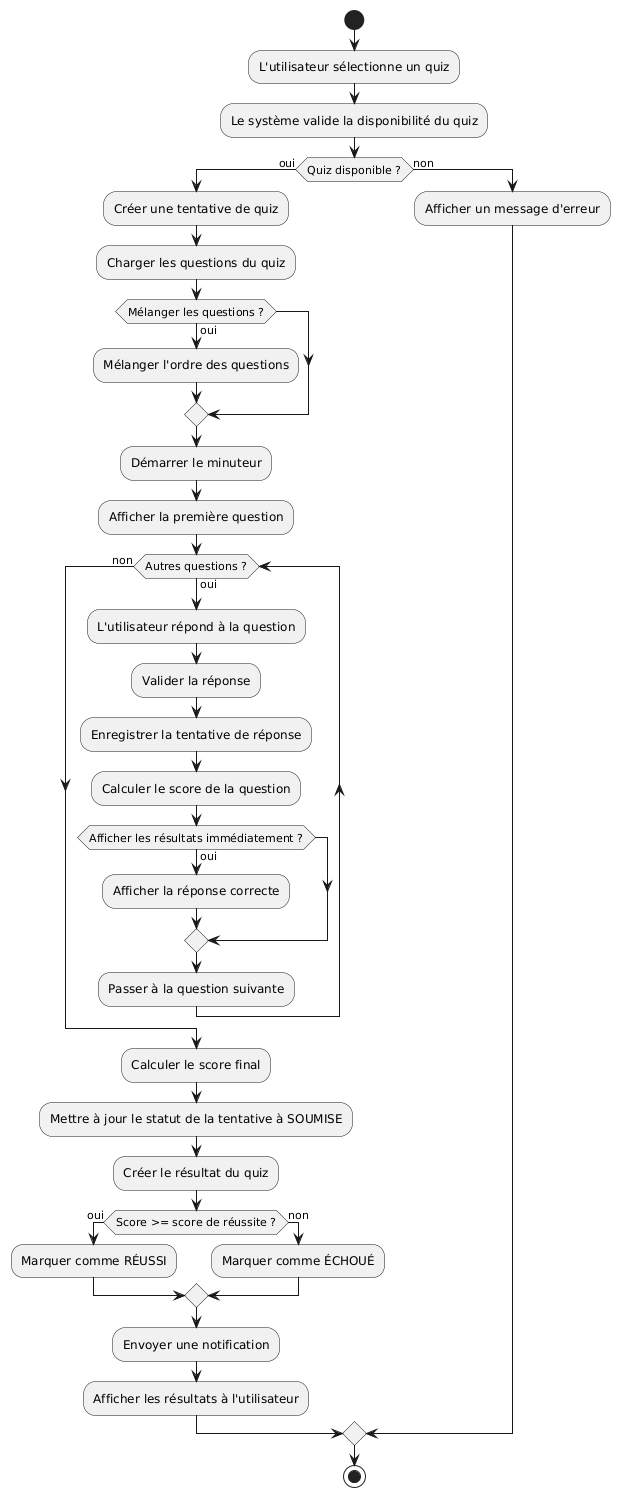
\includegraphics[width=0.8\textwidth]{latex_media/media/activity_diagramme_passer_quiz.png}
    \caption{Diagramme d'activité : Processus de passage d'un quiz}
    \label{fig:activite-passer-quiz}
\end{figure}

Ce diagramme détaille le processus complet de passage d'un quiz, depuis la sélection du quiz par l'utilisateur jusqu'à l'affichage des résultats finaux. Il met en évidence les points de décision critiques, les boucles de traitement des questions, et les différents chemins possibles selon les actions de l'utilisateur.

\subsection{Diagrammes d'état}

Les diagrammes d'état modélisent les différents états que peuvent prendre les objets du système et les transitions entre ces états en réponse aux événements.

\subsubsection{Diagramme d'état : Statut du Quiz}

\begin{figure}[htbp]
    \centering
    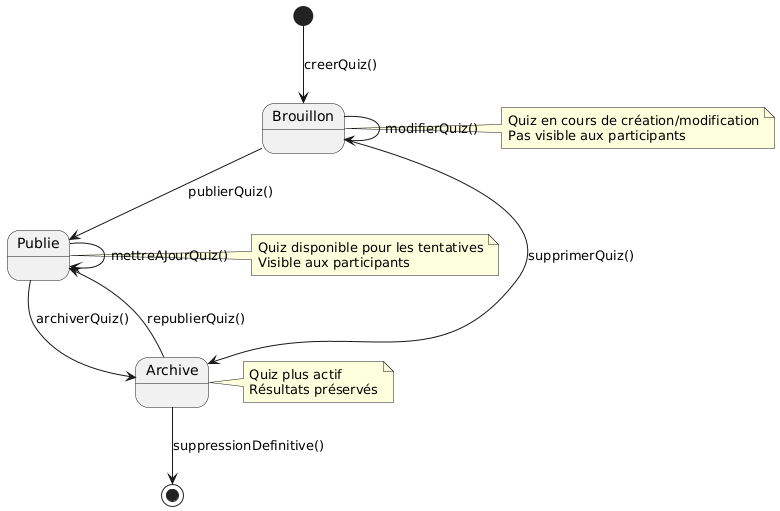
\includegraphics[width=0.8\textwidth]{latex_media/media/Diagrammedetat-StatutduQuiz.png}
    \caption{Diagramme d'état : Cycle de vie d'un quiz}
    \label{fig:etat-statut-quiz}
\end{figure}

Ce diagramme illustre les différents états par lesquels passe un quiz durant son cycle de vie : depuis sa création en mode "Brouillon", sa publication, jusqu'à son archivage final.

\subsubsection{Diagramme d'état : Tentative de Quiz}

\begin{figure}[htbp]
    \centering
    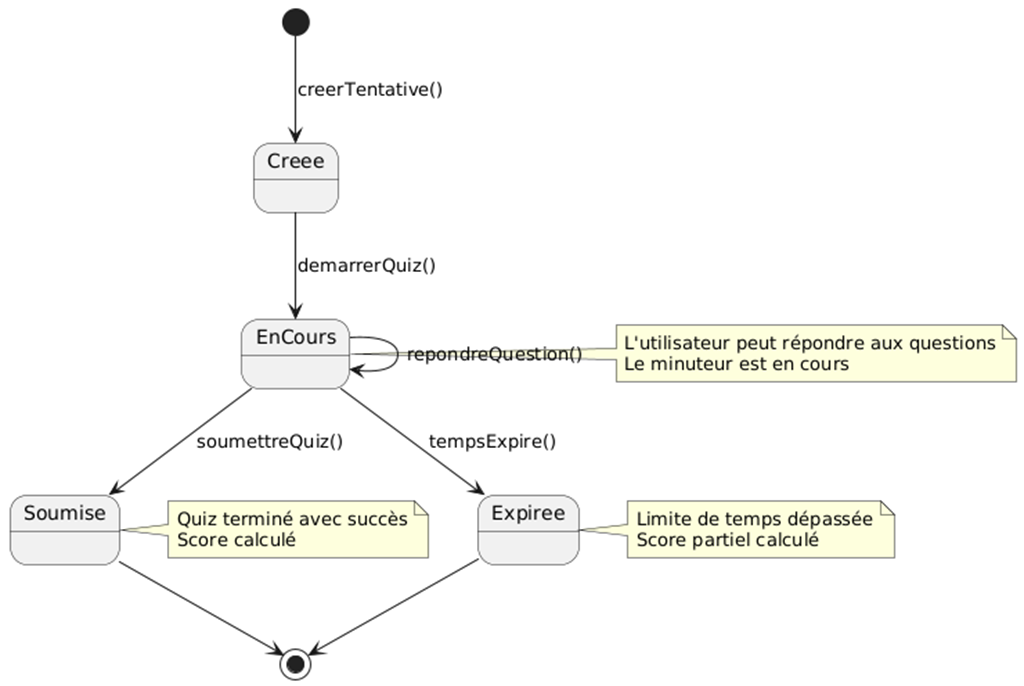
\includegraphics[width=0.8\textwidth]{latex_media/media/Diagrammedetat-Tentative de Quiz.png}
    \caption{Diagramme d'état : États d'une tentative de quiz}
    \label{fig:etat-tentative-quiz}
\end{figure}

Ce diagramme modélise les états d'une tentative de quiz, de sa création jusqu'à son état final (soumise ou expirée), en passant par l'état "en cours" où l'utilisateur répond aux questions.

\subsection{Cartographie fonctionnelle}

La cartographie fonctionnelle présente une vue d'ensemble des principales fonctionnalités du système Quiz Agile et leurs relations dans une perspective de conception.

\begin{figure}[H]
\centering
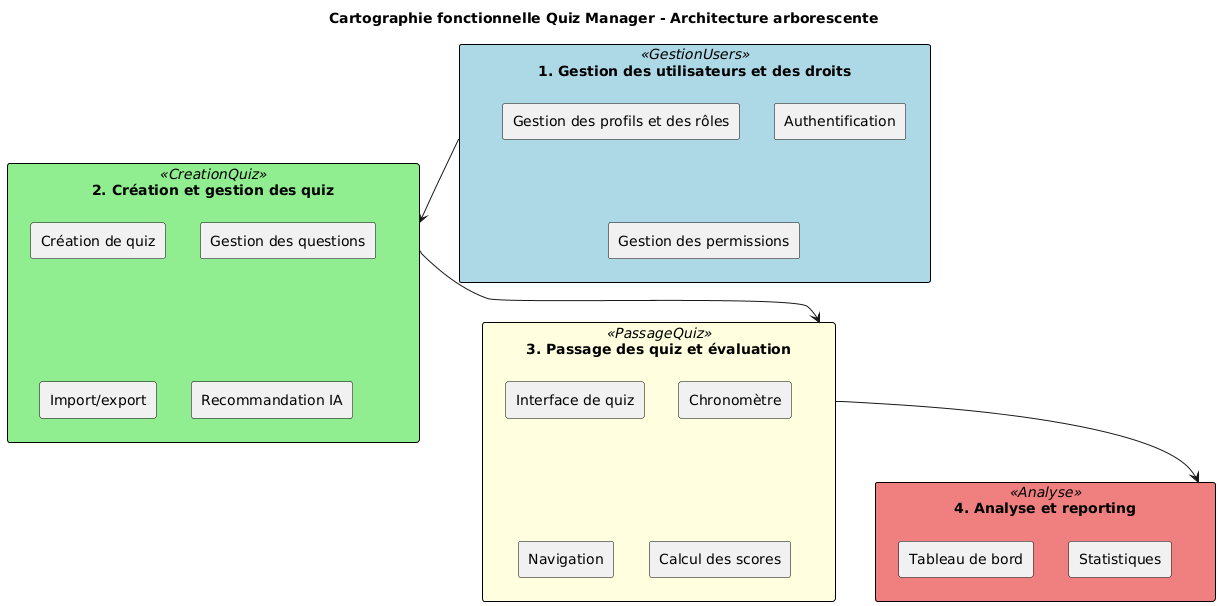
\includegraphics[width=0.8\textwidth]{latex_media/media/image11.png}
\caption{Cartographie fonctionnelle du système Quiz Agile}
\label{fig:cartographie-fonctionnelle}
\end{figure}

Cette cartographie met en évidence les quatre grands modules fonctionnels du système :
\begin{itemize}
\item Module de gestion des utilisateurs et des droits
\item Module de création et gestion des quiz
\item Module de passage des quiz et évaluation
\item Module d'analyse et de reporting
\end{itemize}

\section{Modèle de données}

\subsection{Modèle conceptuel - Diagramme entité-relation}

Le diagramme entité-relation (ERD) présente la structure de données de notre système Quiz Agile, illustrant les entités principales, leurs attributs et les relations qui les lient. Cette modélisation conceptuelle constitue le fondement de notre base de données et assure la cohérence des informations stockées.

\begin{figure}[htbp]
    \centering
    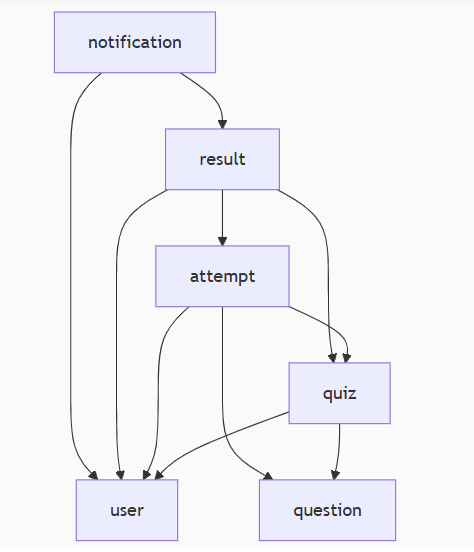
\includegraphics[width=0.85\textwidth]{latex_media/media/Diagramme entite-relation.png}
    \caption{Diagramme entité-relation du système Quiz Agile}
    \label{fig:erd-quiz-agile}
\end{figure}

\subsubsection{Explications des dépendances}

\textbf{Quiz dépend de :}
\begin{itemize}
    \item \textbf{User} (pour le créateur du quiz) - Chaque quiz est créé par un utilisateur spécifique
    \item \textbf{Question} (pour les questions incluses) - Un quiz contient une collection de questions
\end{itemize}

\textbf{Attempt dépend de :}
\begin{itemize}
    \item \textbf{Quiz} (quel quiz est tenté) - Chaque tentative est liée à un quiz spécifique
    \item \textbf{User} (qui tente) - Identifie l'utilisateur qui passe le quiz
    \item \textbf{Question} (pour validation) - Permet de valider les réponses données
\end{itemize}

\textbf{Result agrège les données de :}
\begin{itemize}
    \item \textbf{Quiz} (paramètres) - Récupère les paramètres de notation du quiz
    \item \textbf{User} (participant) - Identifie le participant pour lequel le résultat est généré
    \item \textbf{Attempt} (détails) - Compile les détails de la tentative pour calculer le score
\end{itemize}

\textbf{Notification utilise :}
\begin{itemize}
    \item \textbf{User} (destinataire) - Définit qui recevra la notification
    \item \textbf{Result} (contenu) - Utilise les résultats pour personnaliser le contenu de la notification
\end{itemize}

\subsubsection{Analyse Architecturale}

\begin{itemize}
    \item \textbf{Architecture :} Hexagonale (Domain-Centric) - Cette approche place le domaine métier au centre, isolant la logique business des détails techniques
    \item \textbf{Niveau de couplage :} Modulaire - Les composants sont faiblement couplés, facilitant la maintenance et l'évolution du système
\end{itemize}

Cette architecture garantit une séparation claire des responsabilités et facilite l'évolutivité du système, permettant d'ajouter de nouvelles fonctionnalités sans impacter l'architecture existante.

\subsection{Mécanismes d'import/export}

La conception du système intègre des mécanismes sophistiqués pour l'import et l'export de données, facilitant l'interopérabilité avec d'autres systèmes.

\begin{figure}[H]
\centering
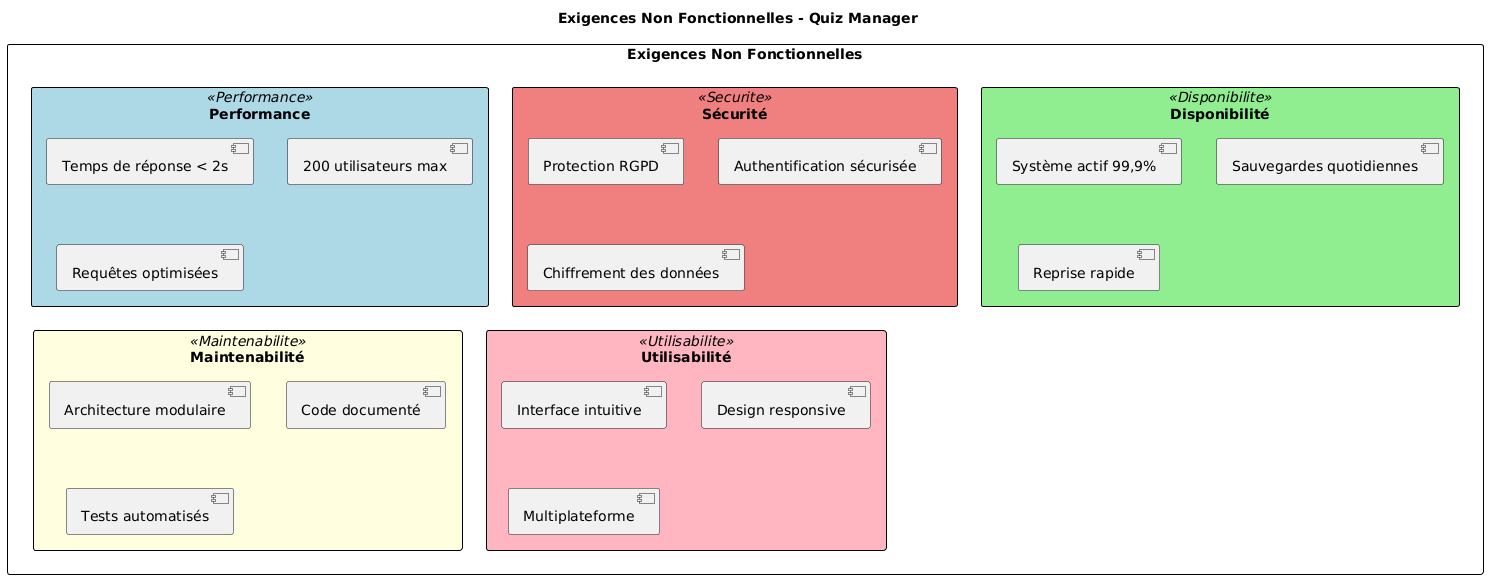
\includegraphics[width=0.9\textwidth]{latex_media/media/image12.png}
\caption{Mécanismes d'import/export de données}
\label{fig:import-export-donnees}
\end{figure}

Ces mécanismes permettent :
\begin{itemize}
\item Import de questions en lot depuis des fichiers CSV ou JSON
\item Export des résultats dans différents formats (PDF, Excel, JSON)
\item Synchronisation avec des systèmes externes via API REST
\item Sauvegarde et restauration de données complètes
\end{itemize}

\subsection{Diagramme de planification du projet}

La planification du projet est représentée par le diagramme de Gantt, qui fait la répartition des tâches sur la période du projet et guide l'implémentation de la conception.

\begin{figure}[H]
\centering
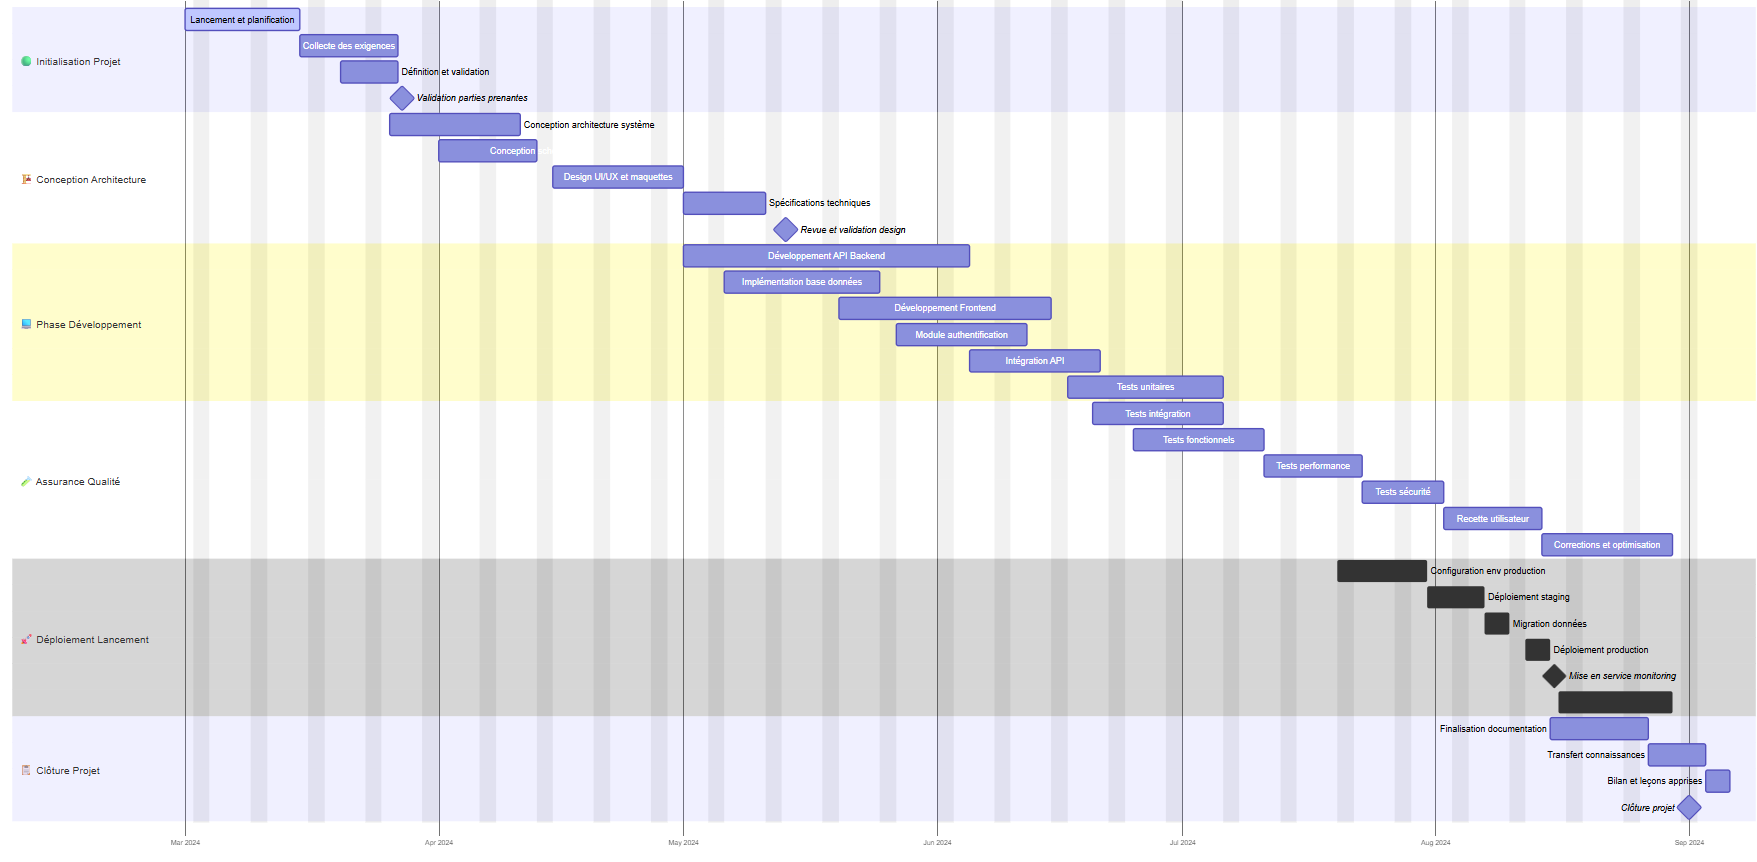
\includegraphics[width=0.9\textwidth]{latex_media/media/image10.png}
\caption{Diagramme de GANTT du projet Quiz Agile}
\label{fig:gantt-quiz-agile}
\end{figure}

Ce diagramme montre la planification détaillée des différentes phases du projet, incluant la conception, le développement, les tests et la validation client. La méthodologie agile Scrum permet une approche itérative avec des cycles de développement courts appelés "sprints", favorisant l'adaptabilité et la réactivité face aux changements de besoins.

\section{Modèle de données}

\subsection{Modèle conceptuel}

Le modèle conceptuel de données définit les entités principales et leurs relations :

\begin{itemize}
    \item Un utilisateur peut créer plusieurs quiz
    \item Un quiz contient plusieurs questions
    \item Une question peut avoir plusieurs réponses
    \item Un utilisateur peut passer plusieurs quiz
    \item Chaque passage génère un résultat
\end{itemize}

\subsection{Modèle relationnel}

Le modèle relationnel dérive du modèle conceptuel et respecte les formes normales pour éviter la redondance et garantir l'intégrité des données.

\section{Technologies et outils utilisés}

\subsection{Backend - Spring Boot}

Spring Boot a été choisi pour le développement du backend pour ses avantages :

\begin{itemize}
    \item Framework mature et robuste
    \item Configuration automatique
    \item Écosystème riche (Spring Security, Spring Data, etc.)
    \item Support natif des API REST
    \item Facilité de test et de déploiement
\end{itemize}

\subsection{Frontend - React}

React a été sélectionné pour l'interface utilisateur :

\begin{itemize}
    \item Composants réutilisables
    \item Virtual DOM pour les performances
    \item Écosystème riche de bibliothèques
    \item Communauté active et documentation complète
\end{itemize}

\subsection{Base de données - MySQL}

MySQL a été choisi comme SGBD relationnel :

\begin{itemize}
    \item Fiabilité et performance éprouvées
    \item Support transactionnel complet
    \item Outils d'administration matures
    \item Compatibilité avec Spring Data JPA
\end{itemize}

\section{Architecture monolithique}

Dans les projets informatiques, une des premières grandes étapes techniques consiste à faire des choix architecturaux : « Comment organiser l'application ? » Deux solutions architecturales principales se présentent : l'architecture monolithique et l'architecture micro-services.

L'architecture monolithique consiste à développer l'application comme une unité unique, où tous les composants sont interconnectés et déployés ensemble. Cette approche peut simplifier le développement initial et la gestion des déploiements, mais elle peut devenir difficile à maintenir et à faire évoluer à mesure que l'application croît.

En revanche, l'architecture micro-services divise l'application en services indépendants, chacun responsable d'une fonctionnalité spécifique. Cela permet une plus grande flexibilité, une scalabilité améliorée et une meilleure gestion des équipes, car chaque service peut être développé, déployé et mis à jour indépendamment.

\begin{figure}[H]
\centering
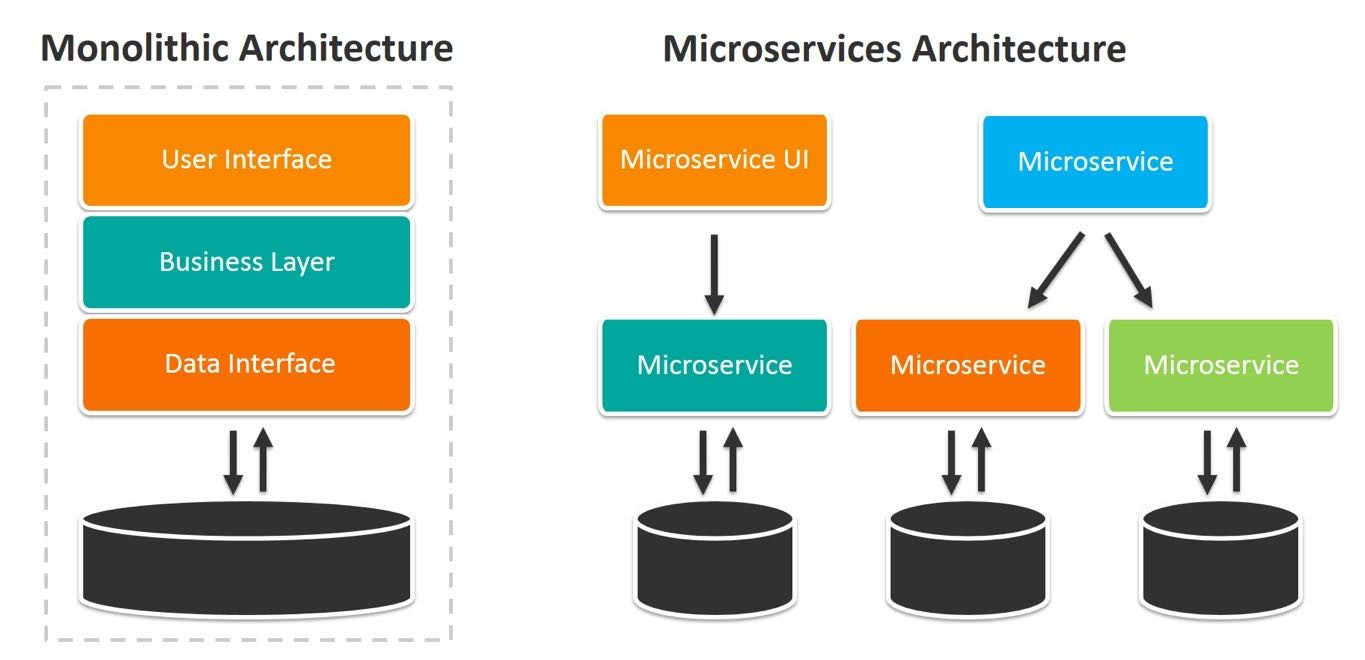
\includegraphics[width=0.8\textwidth]{latex_media/media/image15.jpeg}
\caption{Comparaison entre architecture monolithique et microservices}
\label{fig:comparaison-architectures}
\end{figure}

Pour le cas de la solution QUIZ AGILE, nous avons opté pour l'architecture monolithique. Ce choix nous permet, durant les premières phases du projet, de simplifier la charge cognitive liée à la gestion du code et au déploiement. En structurant l'application comme une unité unique, nous pouvons livrer tout le contenu du monolithe à la fois, ce qui facilite le processus de développement et réduit les complexités associées à l'intégration continue.

Cette approche initiale nous offre également une vue d'ensemble cohérente du projet, permettant aux équipes de se concentrer sur l'implémentation des fonctionnalités sans se soucier des défis d'architecture distribuée. À mesure que le projet évolue et que les besoins se précisent, nous pourrons envisager une transition vers une architecture micro-services si nécessaire.

Le choix d'une architecture monolithique pour cette première phase du projet se justifie par sa simplicité de déploiement et de maintenance, tout en restant compatible avec une éventuelle migration vers une architecture micro-services si les besoins évoluent (scalabilité, modularité accrue).

\section{Conclusion}

Ce chapitre a présenté la conception détaillée du système Quiz Agile, depuis l'architecture générale jusqu'aux choix technologiques. Cette approche structurée garantit un système cohérent, maintenable et évolutif, répondant aux exigences fonctionnelles et non-fonctionnelles identifiées.

% ============================================
% CHAPITRE 4 - Réalisation, Tests et Étude Technique
% ============================================

\cleardoublepage
\thispagestyle{empty}
\begin{center}
    \vspace*{4cm}
    {\Huge \textbf{Chapitre 4}}\\[1.5cm]
    {\LARGE \textbf{Réalisation, Tests et Étude Technique}}
\end{center}
\cleardoublepage

\refstepcounter{chapter}
\addcontentsline{toc}{chapter}{Chapitre \thechapter: Réalisation, Tests et Étude Technique}
\markboth{Chapitre \thechapter: Réalisation, Tests et Étude Technique}{}
\setcounter{section}{0}

\section{Introduction}

Ce chapitre présente la réalisation concrète du projet \textbf{QUIZ AGILE}, en commençant par l'architecture technique adoptée et les choix technologiques qui en découlent. Nous détaillerons ensuite l'implémentation des différents modules, l'environnement de développement mis en place, ainsi que les tests effectués pour valider la solution.

\section{Architecture technique du système}

\subsection{Vue d'ensemble de l'architecture}

L'architecture technique de notre solution Quiz Agile repose sur une approche moderne et structurée qui sépare clairement les responsabilités entre le frontend et le backend. Cette architecture en couches garantit une maintenabilité optimale et facilite les évolutions futures du système.

\begin{figure}[H]
\centering
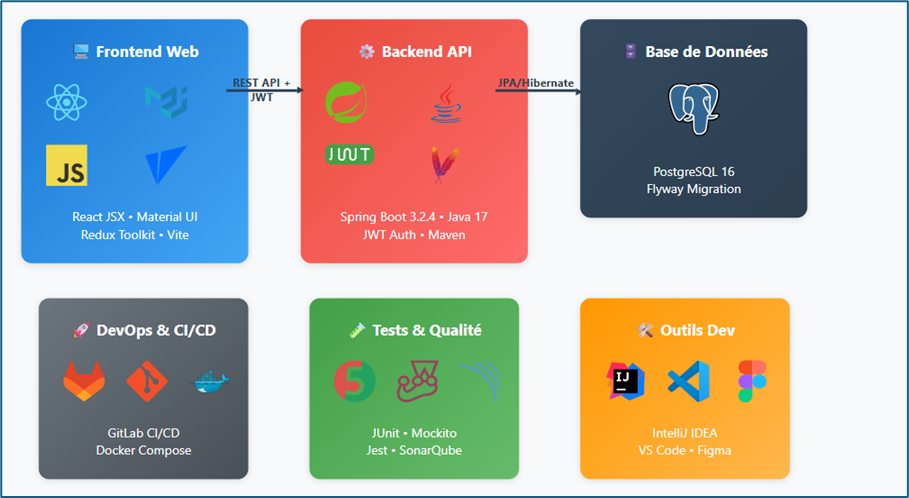
\includegraphics[width=0.9\textwidth]{latex_media/media/architecture_technique_systeme.png}
\caption{Architecture technique du système Quiz Agile}
\label{fig:architecture-technique}
\end{figure}

Le système s'articule autour de trois couches principales :

\begin{itemize}
    \item \textbf{Couche présentation} : Interface utilisateur développée en React avec Material-UI
    \item \textbf{Couche logique métier} : API REST développée avec Spring Boot
    \item \textbf{Couche données} : Base de données PostgreSQL avec Spring Data JPA
\end{itemize}

\subsection{Justification des choix architecturaux}

Le choix d'une architecture monolithique modulaire se justifie par plusieurs facteurs :

\begin{itemize}
    \item \textbf{Simplicité de développement} : Une base de code unifiée facilite la compréhension globale du système
    \item \textbf{Déploiement simplifié} : Une seule application à déployer et monitorer
    \item \textbf{Performance optimale} : Absence de latence réseau entre les modules
    \item \textbf{Cohérence transactionnelle} : Gestion native des transactions ACID
    \item \textbf{Équipe de développement réduite} : Adapté au contexte d'un projet de stage avec ressources limitées
\end{itemize}

Cette approche nous permet de nous concentrer sur la logique métier tout en gardant la flexibilité d'évoluer vers une architecture microservices si les besoins futurs l'exigent.

\section{Environnement de développement}

\subsection{Configuration de l'environnement}

L'environnement de développement a été configuré avec les outils suivants :

\begin{itemize}
    \item \textbf{IDE} : IntelliJ IDEA pour le backend, Visual Studio Code pour le frontend
    \item \textbf{Java} : Version 11 LTS
    \item \textbf{Node.js} : Version 16 LTS
    \item \textbf{Base de données} : MySQL 8.0
    \item \textbf{Outils de build} : Maven pour Java, npm pour React
\end{itemize}

\subsection{Structure du projet}

Le projet est organisé en deux modules principaux :

\begin{itemize}
    \item \textbf{quiz-agile-backend} : Application Spring Boot
    \item \textbf{quiz-agile-frontend} : Application React
\end{itemize}

\section{Implémentation du backend}

\subsection{Configuration Spring Boot}

Le backend utilise Spring Boot avec les dépendances suivantes :

\begin{itemize}
    \item Spring Web (pour les API REST)
    \item Spring Data JPA (pour l'accès aux données)
    \item Spring Security (pour l'authentification)
    \item MySQL Connector (pour la base de données)
    \item Validation API (pour la validation des données)
\end{itemize}

\subsection{Modèle de données}

Les entités principales du système ont été implémentées avec JPA :

\begin{itemize}
    \item Entité User pour la gestion des utilisateurs
    \item Entité Quiz pour les questionnaires
    \item Entité Question pour les questions
    \item Entité Answer pour les réponses
    \item Entité Result pour les résultats
\end{itemize}

\subsection{Services métier}

Les services métier implémentent la logique applicative :

\begin{itemize}
    \item UserService pour la gestion des utilisateurs
    \item QuizService pour la gestion des quiz
    \item QuestionService pour la gestion des questions
    \item ResultService pour l'analyse des résultats
\end{itemize}

\subsection{API REST}

L'API REST expose les fonctionnalités via des contrôleurs :

\begin{itemize}
    \item AuthController pour l'authentification
    \item QuizController pour la gestion des quiz
    \item UserController pour la gestion des utilisateurs
    \item ResultController pour l'accès aux résultats
\end{itemize}

\section{Implémentation du frontend}

\subsection{Architecture React}

L'application frontend est structurée avec :

\begin{itemize}
    \item Composants fonctionnels avec React Hooks
    \item React Router pour la navigation
    \item Axios pour les appels API
    \item Material-UI pour l'interface utilisateur
\end{itemize}

\subsection{Gestion d'état}

La gestion d'état utilise :

\begin{itemize}
    \item Context API pour l'état global
    \item useState et useEffect pour l'état local
    \item Custom hooks pour la logique réutilisable
\end{itemize}

\subsection{Composants principaux}

Les composants principaux incluent :

\begin{itemize}
    \item Dashboard pour le tableau de bord
    \item QuizForm pour la création/édition de quiz
    \item QuizPlayer pour le passage des quiz
    \item ResultsView pour l'affichage des résultats
\end{itemize}

\section{Tests et validation}

\subsection{Tests unitaires}

Des tests unitaires ont été implémentés pour :

\begin{itemize}
    \item Les services métier du backend
    \item Les composants React
    \item Les utilitaires et fonctions helper
\end{itemize}

\subsection{Tests d'intégration}

Les tests d'intégration couvrent :

\begin{itemize}
    \item Les API REST
    \item L'accès aux données
    \item Les flux end-to-end principaux
\end{itemize}

\subsection{Tests de performance}

Des tests de charge ont été réalisés pour valider :

\begin{itemize}
    \item La capacité de traitement concurrent
    \item Les temps de réponse sous charge
    \item La stabilité du système
\end{itemize}

\section{Déploiement}

\subsection{Conteneurisation}

L'application a été conteneurisée avec Docker :

\begin{itemize}
    \item Image Docker pour le backend Spring Boot
    \item Image Docker pour le frontend React buildé
    \item Docker Compose pour l'orchestration locale
\end{itemize}

\subsection{Pipeline CI/CD}

Un pipeline CI/CD a été mis en place avec :

\begin{itemize}
    \item Build automatique sur commit
    \item Exécution des tests automatisés
    \item Déploiement automatique en environnement de test
\end{itemize}

\section{Conclusion}

Ce chapitre a détaillé l'implémentation complète du système Quiz Agile. L'approche méthodique adoptée, combinée aux bonnes pratiques de développement et aux tests rigoureux, a permis de livrer une solution robuste et fonctionnelle répondant aux exigences définies.

\section{Technologies et outils utilisés}

Cette section présente les principales technologies utilisées pour développer la solution Quiz Agile, tant du côté backend que frontend.

\subsection{Backend - Spring Boot}

Spring Boot constitue le cœur de notre architecture backend. Ce framework Java simplifie considérablement le développement d'applications d'entreprise en fournissant une configuration automatique et des modules prêts à l'emploi.

\begin{itemize}
    \item Spring Boot Starter Web : Développement d'API REST
    \item Spring Boot Starter Data JPA : Accès aux données
    \item Spring Boot Starter Security : Sécurité et authentification
    \item Spring Boot Starter Validation : Validation des données
    \item Spring Boot Starter Actuator : Monitoring et santé applicative
    \item Spring Boot Starter Cache : Mise en cache
\end{itemize}

\subsection{Frontend - React}

React est un cadre logiciel d'interface utilisateur open-source créé par Meta Platforms, Inc. Il est utilisé pour développer des applications pour Android, Android TV, iOS, macOS, tvOS, Web, Windows et UWP en permettant aux développeurs d'utiliser le framework React avec les capacités de la plateforme native.

\begin{figure}[H]
\centering

\includegraphics[width=0.5\textwidth]{latex_media/media/image24.png}
\caption{Logo React}
\label{fig:logo-react}
\end{figure}

\subsubsection{Configuration technique du projet}

\begin{itemize}
\item \textbf{Version} : React 19.0.0
\item \textbf{Bibliothèques principales} :
  \begin{itemize}
  \item Material-UI (MUI) 5.15.11 : Composants UI modernes
  \item Redux Toolkit 2.8.2 : Gestion d'état centralisée
  \item React Router DOM 6.22.2 : Navigation côté client
  \item React Redux 9.2.0 : Intégration React-Redux
  \item Axios 1.6.7 : Communication http
  \end{itemize}
\end{itemize}

\subsection{Authentification et Sécurité}

Notre projet utilise une approche moderne de sécurité avec JWT (JSON Web Tokens) intégré à Spring Security :

\subsubsection{JWT (JSON Web Token)}

Le JWT (JSON Web Token) est un jeton sécurisé utilisé pour authentifier un utilisateur dans une application web. Il contient des informations codées (comme l'identifiant de l'utilisateur) et permet de vérifier l'identité de l'utilisateur sans avoir à stocker une session côté serveur.

\subsubsection{Configuration technique du projet}

\begin{itemize}
\item \textbf{Version} : jjwt 0.12.5
\item \textbf{Fonctionnalités} :
  \begin{itemize}
  \item Authentification stateless
  \item Gestion des rôles et permissions
  \item Tokens sécurisés avec signature
  \item Expiration automatique des sessions
  \end{itemize}
\end{itemize}

\begin{figure}[H]
\centering

\includegraphics[width=0.7\textwidth]{latex_media/media/image25.png}
\caption{Logo JWT (JSON Web Token)}
\label{fig:logo-jwt}
\end{figure}

\subsection{Documentation et API}

\subsubsection{SpringDoc OpenAPI}

SpringDoc OpenAPI est une bibliothèque Java qui automatise la génération de documentation API pour les applications Spring Boot. Elle simplifie grandement la documentation des API REST en générant automatiquement des spécifications OpenAPI 3.0 à partir du code source.

\begin{itemize}
\item \textbf{Version} : 2.4.0
\item \textbf{Fonctionnalités} :
  \begin{itemize}
  \item Documentation API automatique basée sur les annotations
  \item Interface Swagger UI interactive pour tester les endpoints
  \item Génération de schémas OpenAPI 3.0 complets
  \item Tests d'API intégrés avec interface utilisateur intuitive
  \item Support des modèles de données complexes et des validations
  \end{itemize}
\end{itemize}

SpringDoc OpenAPI analyse automatiquement les contrôleurs REST et génère une documentation complète incluant les paramètres, les types de retour, les codes de statut HTTP et les exemples de requêtes/réponses. Cette approche garantit que la documentation reste toujours synchronisée avec le code source.

\subsubsection{Monitoring et Observabilité}

\paragraph{Spring Boot Actuator}

Spring Boot Actuator fournit des fonctionnalités de production prêtes à l'emploi pour surveiller et gérer notre application Quiz Agile. Il expose des endpoints de gestion qui permettent de monitorer l'état de santé de l'application et de collecter des métriques importantes.

Les principales fonctionnalités incluent :
\begin{itemize}
    \item \textbf{Health checks} : Vérification automatique de l'état de l'application, de la base de données et des services externes
    \item \textbf{Métriques} : Monitoring des performances avec des métriques détaillées sur les requêtes, la mémoire, les threads et les connexions
    \item \textbf{Endpoints} : Points d'accès REST pour le monitoring externe (/actuator/health, /actuator/metrics, /actuator/info)
    \item \textbf{Info} : Informations détaillées sur l'application, la version, l'environnement et la configuration
\end{itemize}

\paragraph{Système de mise en cache}

Notre architecture intègre un système de cache sophistiqué pour optimiser les performances :

\begin{itemize}
    \item \textbf{Spring Cache} : Mise en cache transparente des données fréquemment accédées avec des annotations déclaratives
    \item \textbf{Amélioration des performances} : Réduction significative des accès à la base de données pour les opérations de lecture fréquentes
    \item \textbf{Cache intelligent} : Invalidation automatique du cache lors des modifications de données
    \item \textbf{Stratégies de cache} : Support de différentes stratégies (LRU, FIFO) adaptées aux besoins spécifiques
\end{itemize}

\subsection{Base de données}

\subsubsection{PostgreSQL}

\textbf{PostgreSQL} est un système de gestion de base de données relationnelle (SGBDR) open-source avancé. Une base de données relationnelle organise les données en une ou plusieurs tables de données dans lesquelles les données peuvent être reliées les unes aux autres ; ces relations aident à structurer les données.

\subsubsection{Configuration technique du projet}

\begin{itemize}
\item \textbf{Version} : PostgreSQL 16-alpine
\item \textbf{Migration} : Flyway pour la gestion des schémas
\item \textbf{Connexion} : Pool de connexions optimisé
\item \textbf{Tests} : H2 Database pour les tests unitaires
\end{itemize}

\begin{figure}[H]
\centering

\includegraphics[width=0.6\textwidth]{latex_media/media/image26.png}
\caption{Logo PostgreSQL}
\label{fig:logo-postgresql}
\end{figure}

\subsection{Système de gestion de dépendances}

Aujourd'hui des milliers, si pas des billions de packages sont publiés chaque jour par des développeurs passionnés partout dans le monde et dans différents langages de programmation. Ces packages ou modules sont tout simplement des lignes de codes qui permettent de remplir une certaine fonctionnalité et qui peuvent être importées et utilisées répétitivement. Et comme c'est le cas pour tous les projets de logiciel, on n'allait pas réinventer la roue, et on faisait appel à ces dépendances. Le problème qui se pose alors est dans la gestion de ces derniers, et de leurs différentes versions.

C'est pourquoi on fait recours à des outils de gestion de paquets/dépendances notamment npm pour JavaScript, et maven pour java.

\subsubsection{Maven}

Maven est un outil de gestion et de compréhension de projet open source principalement utilisé pour les projets Java. Maven peut également être utilisé pour construire et gérer des projets écrits en C\#, Ruby, Scala et d'autres langages.

Maven utilise un modèle d'objet de projet (POM) et un ensemble de plugins pour gérer la construction, la génération de rapports et la documentation d'un projet à partir d'une information centrale.

\begin{figure}[htbp]
    \centering
    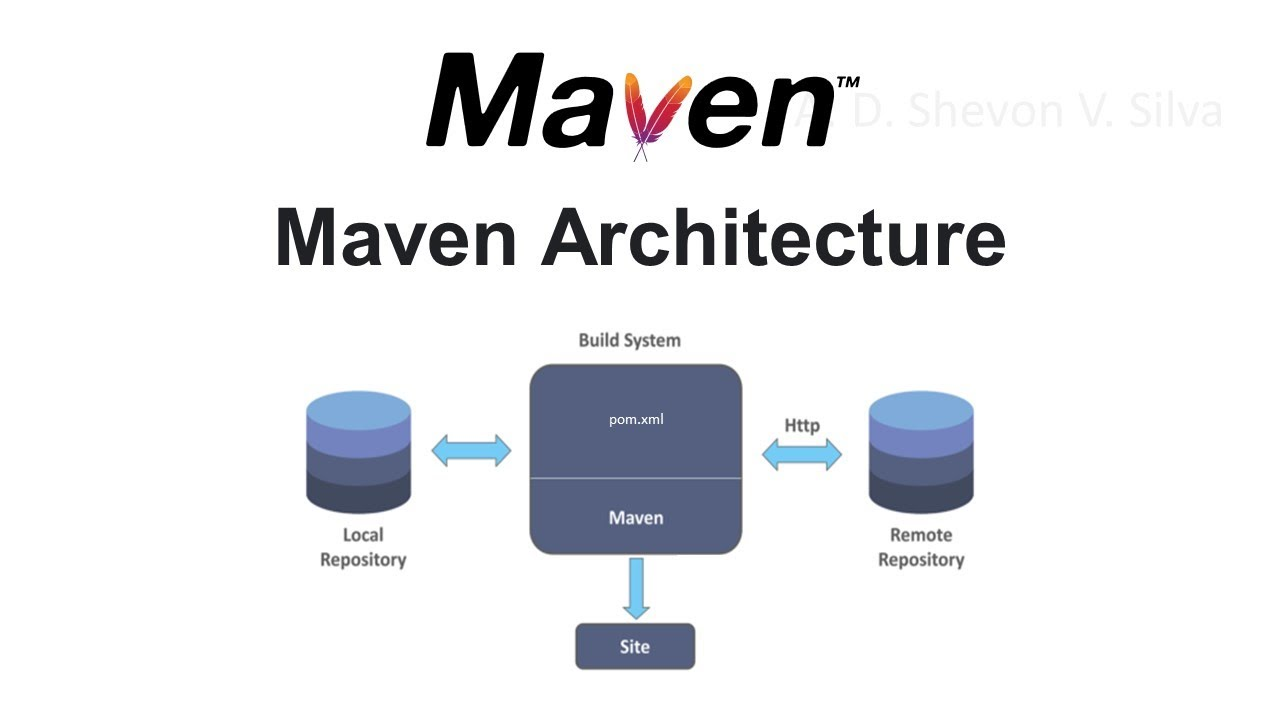
\includegraphics[width=0.8\textwidth]{latex_media/media/maven.png}
    \caption{Logo et architecture Maven}
    \label{fig:maven-logo}
\end{figure}

Les principales fonctionnalités de Maven incluent :

\begin{itemize}
    \item \textbf{Gestion des dépendances} : Téléchargement automatique des bibliothèques requises
    \item \textbf{Construction standardisée} : Structure de projet uniforme
    \item \textbf{Cycle de vie} : Phases de construction prédéfinies (compile, test, package, install, deploy)
    \item \textbf{Plugins} : Extensions pour des fonctionnalités spécifiques
    \item \textbf{Repositories} : Stockage centralisé des artefacts
\end{itemize}



Le fichier POM.xml (Project Object Model) est le cœur de tout projet Maven. Il contient les informations sur le projet et les détails de configuration utilisés par Maven pour construire le projet, incluant les dépendances, les plugins, les objectifs, les profils de build, la version du projet, la description, et bien plus encore.

\section{Outils de développement et de test}

Cette section présente l'écosystème d'outils de développement, de test et d'intégration continue utilisés dans le projet Quiz Agile. Ces outils garantissent la qualité du code, l'automatisation des tests et la fiabilité du processus de déploiement.

\subsection{Outils de test}

\subsubsection{JUnit 5}

JUnit 5 est le framework de test standard pour Java. Il fournit une approche moderne et flexible pour écrire et exécuter des tests unitaires et d'intégration.

\begin{figure}[htbp]
    \centering
    
\includegraphics[width=0.6\textwidth]{latex_media/media/junit.png}
    \caption{Logo JUnit 5 - Framework de test Java}
    \label{fig:junit-logo}
\end{figure}

JUnit 5 apporte plusieurs améliorations par rapport aux versions précédentes :
\begin{itemize}
    \item \textbf{Architecture modulaire} : Séparation claire entre JUnit Platform, Jupiter et Vintage
    \item \textbf{Annotations nouvelles} : @DisplayName, @ParameterizedTest, @RepeatedTest
    \item \textbf{Assertions améliorées} : Messages d'erreur plus expressifs
    \item \textbf{Tests dynamiques} : Génération de tests à l'exécution
\end{itemize}

\subsubsection{Mockito}

Mockito est un framework de mocking pour Java qui permet de créer des objets simulés (mocks) pour isoler les unités de code lors des tests.

\begin{figure}[htbp]
    \centering
    
\includegraphics[width=0.6\textwidth]{latex_media/media/mockito.png}
    \caption{Logo Mockito - Framework de mocking Java}
    \label{fig:mockito-logo}
\end{figure}

Les principales fonctionnalités de Mockito incluent :
\begin{itemize}
    \item \textbf{Création de mocks} : Simulation d'objets complexes
    \item \textbf{Stubbing} : Définition du comportement des mocks
    \item \textbf{Vérification} : Contrôle des interactions avec les mocks
    \item \textbf{Spy objects} : Objets partiellement mockés
\end{itemize}

\subsubsection{Jest}

Jest est un framework de test JavaScript développé par Meta, optimisé pour tester les applications React et Node.js.

\begin{figure}[htbp]
    \centering
    
\includegraphics[width=0.6\textwidth]{latex_media/media/jest_react_test.png}
    \caption{Jest - Framework de test JavaScript pour React}
    \label{fig:jest-logo}
\end{figure}

Jest offre une expérience de test complète avec :
\begin{itemize}
    \item \textbf{Zero configuration} : Fonctionne out-of-the-box
    \item \textbf{Snapshot testing} : Tests de régression UI
    \item \textbf{Code coverage} : Couverture de code intégrée
    \item \textbf{Mocking puissant} : Système de mocks avancé
\end{itemize}

\subsection{Outils de documentation et modélisation}

\subsubsection{PlantUML}

PlantUML est un outil permettant de créer des diagrammes UML à partir de descriptions textuelles simples.

\begin{figure}[htbp]
    \centering
    
\includegraphics[width=0.6\textwidth]{latex_media/media/plantUML.png}
    \caption{Logo PlantUML - Outil de génération de diagrammes UML}
    \label{fig:plantuml-logo}
\end{figure}

PlantUML facilite la création de :
\begin{itemize}
    \item \textbf{Diagrammes de séquence} : Interactions entre objets
    \item \textbf{Diagrammes de cas d'utilisation} : Modélisation fonctionnelle
    \item \textbf{Diagrammes de classes} : Structure du système
    \item \textbf{Diagrammes d'activité} : Flux de processus
\end{itemize}

\subsection{Outils de test API et intégration}

\subsubsection{Postman}

Postman est une plateforme collaborative pour le développement et le test d'APIs REST.

\begin{figure}[htbp]
    \centering
    
\includegraphics[width=0.6\textwidth]{latex_media/media/postman.png}
    \caption{Logo Postman - Plateforme de test d'API}
    \label{fig:postman-logo}
\end{figure}

Postman permet de :
\begin{itemize}
    \item \textbf{Tester les APIs} : Envoi de requêtes HTTP et validation des réponses
    \item \textbf{Automatisation} : Collections de tests automatisés
    \item \textbf{Documentation} : Génération automatique de documentation API
    \item \textbf{Monitoring} : Surveillance continue des APIs
\end{itemize}

\subsection{Outils DevOps et gestion de version}

\subsubsection{Git}

Git est un système de contrôle de version distribué qui permet de gérer l'historique des modifications du code source de manière efficace et collaborative.

\begin{figure}[htbp]
    \centering
    
\includegraphics[width=0.6\textwidth]{latex_media/media/git.png}
    \caption{Logo Git - Système de contrôle de version distribué}
    \label{fig:git-logo}
\end{figure}

Git offre les fonctionnalités suivantes :
\begin{itemize}
    \item \textbf{Versionning distribué} : Chaque développeur possède une copie complète de l'historique
    \item \textbf{Branches et merges} : Développement parallèle et fusion intelligente
    \item \textbf{Historique complet} : Traçabilité complète des modifications
    \item \textbf{Performance} : Opérations rapides même sur de gros projets
\end{itemize}

\subsubsection{GitLab}

GitLab est une plateforme DevOps complète qui intègre la gestion de code source, l'intégration continue, et le déploiement dans une solution unifiée.

\begin{figure}[htbp]
    \centering
    
\includegraphics[width=0.6\textwidth]{latex_media/media/gitlab.png}
    \caption{Logo GitLab - Plateforme DevOps complète}
    \label{fig:gitlab-logo}
\end{figure}

GitLab propose :
\begin{itemize}
    \item \textbf{Repositories Git} : Gestion centralisée du code source
    \item \textbf{CI/CD intégré} : Pipelines d'intégration et déploiement automatisés
    \item \textbf{Issue tracking} : Gestion des tâches et bugs
    \item \textbf{Code review} : Processus de révision de code avec merge requests
\end{itemize}

\subsubsection{npm}

npm (Node Package Manager) est le gestionnaire de paquets par défaut pour Node.js et l'écosystème JavaScript, utilisé pour gérer les dépendances du frontend React.

\begin{figure}[htbp]
    \centering
    
\includegraphics[width=0.6\textwidth]{latex_media/media/npm.png}
    \caption{Logo npm - Gestionnaire de paquets Node.js}
    \label{fig:npm-logo}
\end{figure}

npm facilite :
\begin{itemize}
    \item \textbf{Gestion des dépendances} : Installation et mise à jour automatique des packages
    \item \textbf{Scripts de build} : Automatisation des tâches de développement
    \item \textbf{Registry central} : Accès à des millions de packages open source
    \item \textbf{Versioning sémantique} : Gestion fine des versions des dépendances
\end{itemize}

\subsubsection{Docker}

Docker est une plateforme de conteneurisation qui permet d'empaqueter les applications et leurs dépendances dans des conteneurs légers et portables.

\begin{figure}[htbp]
    \centering
    
\includegraphics[width=0.6\textwidth]{latex_media/media/docker.png}
    \caption{Logo Docker - Plateforme de conteneurisation}
    \label{fig:docker-logo}
\end{figure}

Docker apporte :
\begin{itemize}
    \item \textbf{Conteneurisation} : Isolation des applications dans des environnements reproductibles
    \item \textbf{Portabilité} : Déploiement identique sur différents environnements
    \item \textbf{Scalabilité} : Orchestration et mise à l'échelle automatique
    \item \textbf{Efficacité} : Utilisation optimisée des ressources système
\end{itemize}

\subsection{Intégration continue et déploiement}

\subsubsection{Jenkins}

Jenkins est un serveur d'automatisation open source qui facilite l'intégration continue et le déploiement continu (CI/CD).

\begin{figure}[htbp]
    \centering
    
\includegraphics[width=0.6\textwidth]{latex_media/media/jenkins.png}
    \caption{Logo Jenkins - Serveur d'intégration continue}
    \label{fig:jenkins-logo}
\end{figure}

Jenkins offre :
\begin{itemize}
    \item \textbf{Automatisation des builds} : Compilation et packaging automatiques
    \item \textbf{Exécution des tests} : Tests automatisés à chaque commit
    \item \textbf{Déploiement automatique} : Pipeline de livraison continue
    \item \textbf{Notifications} : Alertes en cas d'échec ou de succès
\end{itemize}

\subsection{Outils d'analyse de qualité de code}

\subsubsection{SonarQube}

SonarQube est un outil d'analyse statique de code qui évalue automatiquement la qualité, la fiabilité, la sécurité, et la maintenabilité d'un projet. Il prend en charge de nombreux langages (Java, JavaScript, TypeScript, C\#, etc.) et s'intègre dans la chaîne CI/CD pour fournir des rapports en temps réel à chaque build ou pull request.

\begin{figure}[htbp]
    \centering
    
\includegraphics[width=0.6\textwidth]{latex_media/media/sonarqube.png}
    \caption{Logo SonarQube - Plateforme d'analyse de qualité de code}
    \label{fig:sonarqube-logo}
\end{figure}

\textbf{Objectifs de SonarQube :}

SonarQube vise à améliorer continuellement la qualité du code source en identifiant automatiquement les problèmes potentiels et en proposant des recommandations d'amélioration :

\begin{itemize}
    \item \textbf{Détecter les bugs} : Identification automatique des erreurs potentielles et des code smells qui peuvent affecter la maintenabilité
    \item \textbf{Analyser les duplications} : Détection du code dupliqué pour promouvoir la réutilisabilité et réduire la maintenance
    \item \textbf{Identifier les vulnérabilités} : Scan de sécurité pour détecter les failles de sécurité communes (OWASP Top 10)
    \item \textbf{Suivre la couverture de tests} : Intégration avec les outils de test (JaCoCo, Jest...) pour mesurer l'efficacité des tests unitaires
    \item \textbf{Définir des Quality Gates} : Établissement de seuils de qualité minimum à respecter avant toute mise en production
    \item \textbf{Renforcer les bonnes pratiques} : Promotion des standards de développement et amélioration continue des compétences de l'équipe
\end{itemize}

\textbf{Intégration dans le projet Quiz Agile :}

Dans notre projet, SonarQube s'intègre parfaitement dans notre pipeline CI/CD Jenkins pour assurer une qualité de code continue :

\begin{figure}[htbp]
    \centering
    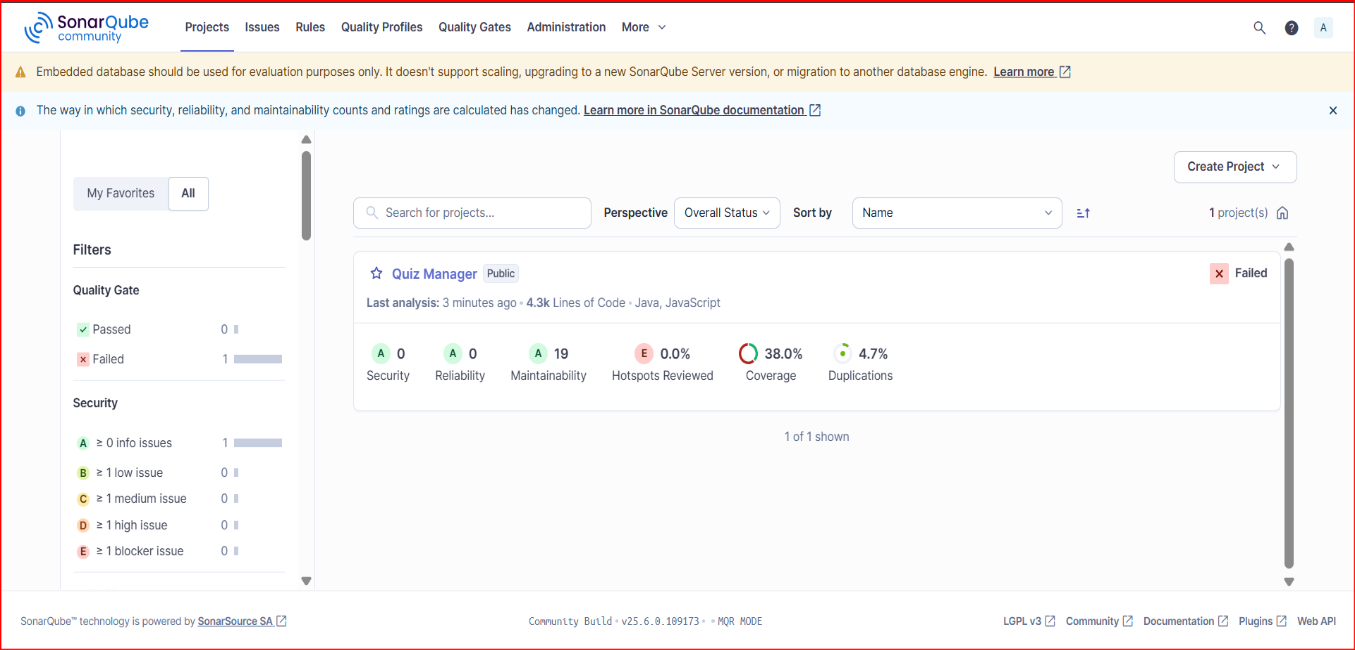
\includegraphics[width=0.85\textwidth]{latex_media/media/Analyse de code avec SonarQube.png}
    \caption{Analyse de code avec SonarQube - Dashboard de qualité du projet Quiz Agile}
    \label{fig:sonarqube-analysis}
\end{figure}

L'analyse SonarQube de notre projet Quiz Agile révèle :
\begin{itemize}
    \item \textbf{Couverture de tests} : Maintien d'un taux de couverture supérieur à 80\% pour le backend Java et 75\% pour le frontend React
    \item \textbf{Complexité cyclomatique} : Respect des seuils recommandés pour maintenir un code lisible et maintenable
    \item \textbf{Vulnérabilités} : Zéro vulnérabilité critique détectée grâce aux bonnes pratiques de sécurité Spring Security et validation des entrées
    \item \textbf{Code smells} : Nombre minimal de code smells maintenus par des revues de code régulières et des refactorings continus
    \item \textbf{Technical debt} : Ratio de dette technique maintenu sous les seuils acceptables définis par l'équipe
\end{itemize}

Cette approche garantit une base de code robuste et facilite la maintenance à long terme du système Quiz Agile.

\section{Architecture technique globale}

\subsection{Vue d'ensemble de la stack technologique}

L'architecture technique de notre solution Quiz Agile repose sur une stack technologique moderne et bien structurée qui couvre l'ensemble du cycle de développement et de déploiement.

\begin{figure}[H]
\centering

\includegraphics[width=1.0\textwidth]{latex_media/media/stack_technologique_quiz_agile.png}
\caption{Stack technologique complète du projet Quiz Agile}
\label{fig:stack-technologique}
\end{figure}

Cette vue d'ensemble illustre la répartition des technologies selon les domaines fonctionnels :

\begin{itemize}
\item \textbf{Frontend Web} : React JSX + Material UI, Redux Toolkit + Vite pour un développement moderne et performant
\item \textbf{Backend API} : Spring Boot 3.2.4 + Java 17 avec JWT Auth + Maven pour une architecture robuste et sécurisée
\item \textbf{Base de Données} : PostgreSQL 16 avec Flyway Migration pour une gestion efficace des données
\item \textbf{DevOps \& CI/CD} : GitLab CI/CD, Docker Compose pour l'automatisation des déploiements
\item \textbf{Tests \& Qualité} : JUnit + Mockito, Jest + SonarQube pour garantir la qualité du code
\item \textbf{Outils Dev} : IntelliJ IDEA, VS Code + Figma pour un environnement de développement optimal
\end{itemize}

\subsection{Architecture technique détaillée}

En guise de conclusion à cette analyse technique, cette section présente globalement l'architecture technique que nous avons adoptée pour mettre en œuvre notre projet QUIZ AGILE. Nous avons choisi une architecture moderne et flexible qui répond aux exigences de performance, de scalabilité et de sécurité.

Cette architecture repose sur des technologies éprouvées, intégrant des composants robustes pour le développement de notre backend avec Spring Boot, et un frontend dynamique grâce à React. L'utilisation de PostgreSQL comme base de données assure une gestion efficace et sécurisée des données, tandis que JWT est intégré pour gérer l'authentification et les autorisations, renforçant ainsi la sécurité globale de la plateforme.

Grâce à ces choix technologiques, nous sommes en mesure de créer une solution cohérente et performante, facilitant la collaboration entre les équipes et améliorant l'expérience utilisateur.

\begin{figure}[H]
\centering
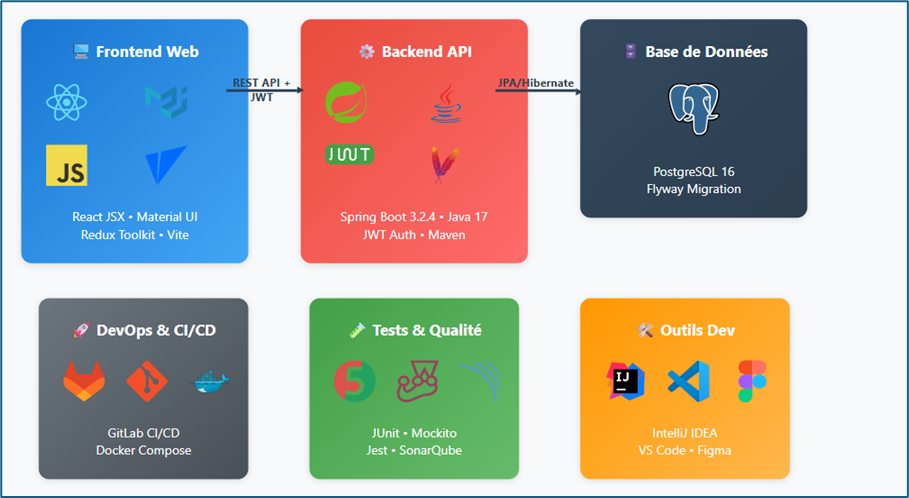
\includegraphics[width=1.0\textwidth]{latex_media/media/architecture_technique_systeme.png}
\caption{Architecture technique de l'application Quiz Agile}
\label{fig:architecture-technique}
\end{figure}

\section{Architecture générale du système}

\subsection{Vue d'ensemble architecturale}

La figure ci-dessous présente l'architecture générale de l'application QUIZ AGILE, mettant en lumière les interactions entre les différentes couches, notamment le front-end, le serveur d'authentification JWT, ainsi que le back-end et la base de données. Cette architecture vise à garantir une communication fluide et sécurisée entre les différentes parties, tout en optimisant les performances globales de l'application.

\begin{figure}[H]
\centering
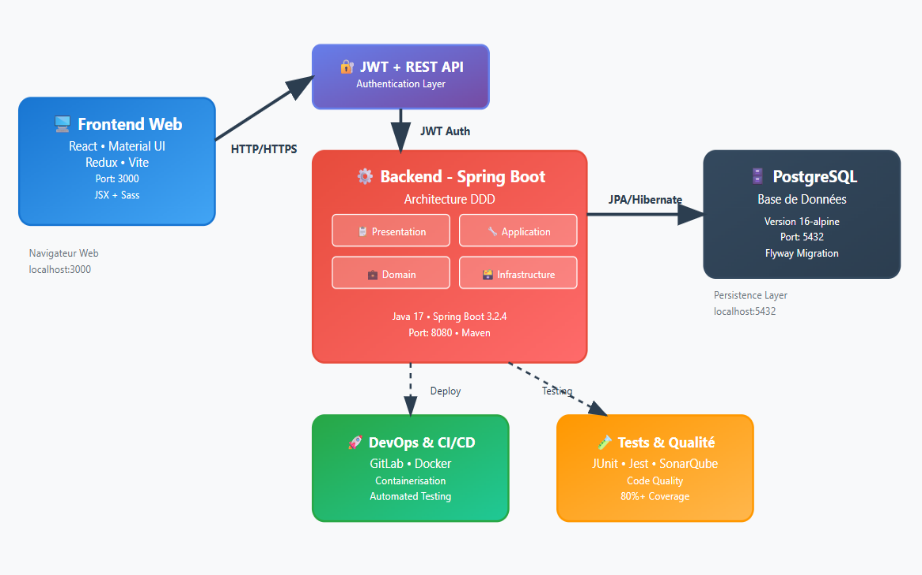
\includegraphics[width=1.0\textwidth]{latex_media/media/Architecture_globale.png}
\caption{Architecture globale de l'application Quiz Agile}
\label{fig:architecture-globale}
\end{figure}

\subsection{Architecture Backend détaillée}

La figure suivante représente l'architecture logicielle du projet Agile Quiz, conçue selon les principes de la Clean Architecture et du modèle DDD (Domain-Driven Design). L'application est organisée en plusieurs couches bien distinctes : la couche de présentation (controllers REST, sécurité, validation), la couche d'application (services, DTOs, mappers), la couche d'infrastructure (repositories JPA, configurations, services externes), et le cœur du domaine (entités, objets de valeur, règles métiers, interfaces).

Cette séparation permet de garantir la modularité, la testabilité, ainsi qu'une meilleure maintenabilité du code. Le backend est développé avec Spring Boot et utilise PostgreSQL comme base de données, tandis que le frontend est construit avec React et Material UI.

\subsection{Structure et implémentation du projet Backend}

\subsubsection{Architecture Domain-Driven Design (DDD)}

Notre backend QUIZ AGILE suit rigoureusement les principes du Domain-Driven Design avec une architecture Clean. Cette approche nous permet de maintenir une séparation claire des responsabilités et une forte cohésion métier.

\paragraph{Organisation des couches}

La partie backend de notre projet QUIZ AGILE est structurée en quatre couches principales, chacune ayant un rôle spécifique dans l'architecture :

\begin{itemize}
\item \textbf{Couche de Sécurité} : Cette couche est responsable de la gestion des authentifications et des autorisations. En intégrant Spring Security avec JWT, elle assure la protection des ressources et le contrôle d'accès, garantissant que seuls les utilisateurs autorisés peuvent interagir avec le système. Elle gère également les rôles utilisateur (ADMIN, COACH, MODERATOR, USER) et les permissions associées.

\item \textbf{Couche DAO (Data Access Object)} : La couche DAO est chargée de l'accès aux données. Elle encapsule la logique nécessaire pour interagir avec la base de données PostgreSQL, facilitant ainsi les opérations de création, lecture, mise à jour et suppression (CRUD). Cette abstraction permet de séparer la logique d'accès aux données de la logique métier et utilise Spring Data JPA pour simplifier les opérations de persistance.

\item \textbf{Couche Service} : La couche service contient la logique métier de l'application. Elle traite les requêtes provenant des contrôleurs, exécute les opérations nécessaires en utilisant les DAOs, et renvoie les résultats. Cette couche assure également la validation des données, la gestion des règles métier, et l'orchestration des différents composants pour répondre aux cas d'usage fonctionnels.

\item \textbf{Couche Contrôleur} : La couche contrôleur agit comme un intermédiaire entre le frontend React et le backend Spring Boot. Elle reçoit les requêtes HTTP REST, les dirige vers les services appropriés, et retourne les réponses au format JSON. Cette couche est essentielle pour gérer le flux des données et assurer une communication fluide entre les différentes parties de l'application.
\end{itemize}

\paragraph{Enrichissement de l'architecture Backend}

Notre architecture backend est enrichie par l'intégration des couches et éléments supplémentaires suivants :

\begin{itemize}
\item \textbf{Configs} : Cette couche contient des fichiers de configuration pour l'application Spring Boot. Elle définit les paramètres globaux comme les connexions à la base de données PostgreSQL, les configurations de sécurité JWT, les propriétés de l'application, et les beans de configuration nécessaires au bon fonctionnement du système.

\item \textbf{DTO (Data Transfer Object)} : Les DTO sont utilisés pour transporter des données entre les différentes couches de l'application et avec le frontend React. Ils permettent de réduire le nombre d'appels entre le frontend et le backend en regroupant plusieurs attributs en un seul objet, tout en offrant une couche d'abstraction pour protéger les entités internes.

\item \textbf{Entities} : Cette couche définit les entités JPA qui correspondent aux tables de la base de données PostgreSQL. Chaque entité (Quiz, User, Question, QuizAttempt, etc.) représente un modèle de données et inclut des annotations JPA pour la validation et la gestion des relations entre les entités.

\item \textbf{Exceptions} : La gestion des exceptions est cruciale pour le traitement des erreurs dans l'application. Cette couche définit des classes d'exception personnalisées pour gérer des cas d'erreurs spécifiques (QuizNotFoundException, UserAlreadyExistsException, etc.), permettant une gestion plus claire et centralisée des erreurs avec des messages appropriés.

\item \textbf{Handlers} : Les handlers traitent des requêtes spécifiques ou des événements de l'application. Ils incluent les gestionnaires d'exceptions globaux (@ControllerAdvice), les handlers d'authentification, et les gestionnaires d'événements pour des flux de travail complexes comme la génération de rapports PDF.

\item \textbf{Mappers} : Les mappers, implémentés avec MapStruct, sont responsables de la conversion entre les entités JPA, les DTO et d'autres représentations de données. Ils facilitent le passage des données entre les différentes couches en s'assurant que les structures de données sont compatibles et en automatisant les conversions.

\item \textbf{Repositories} : Les repositories encapsulent la logique d'accès aux données et interagissent directement avec la base de données PostgreSQL via Spring Data JPA. Ils fournissent une interface pour des opérations CRUD sur les entités, séparant ainsi la logique de persistance de la logique métier et offrant des requêtes personnalisées.

\item \textbf{Responses} : Les objets de réponse contiennent les données que le serveur renvoie au client React. Ils structurent les informations pour une communication claire et efficace, incluant les codes de statut HTTP, les messages d'erreur, et les données de réponse formatées.
\end{itemize}

\paragraph{Intégration et cohérence architecturale}

Ces couches et éléments travaillent ensemble pour créer une architecture backend robuste et maintenable. L'utilisation de Spring Boot comme framework principal assure une intégration fluide entre tous les composants, tandis que les annotations Spring facilitent la configuration et l'injection de dépendances.

L'architecture suit les principes de séparation des responsabilités et de faible couplage, permettant une évolution et une maintenance aisées du système. Les tests unitaires et d'intégration sont intégrés à chaque couche pour garantir la qualité et la fiabilité du code.

Cette structure facilite également la collaboration en équipe, chaque développeur pouvant travailler sur une couche spécifique sans impacter les autres, tout en maintenant une cohérence globale grâce aux interfaces bien définies entre les couches.

\paragraph{Structure physique du projet Backend}

La structure physique de notre projet backend Spring Boot reflète parfaitement l'organisation architecturale décrite ci-dessus :

\begin{figure}[H]
\centering
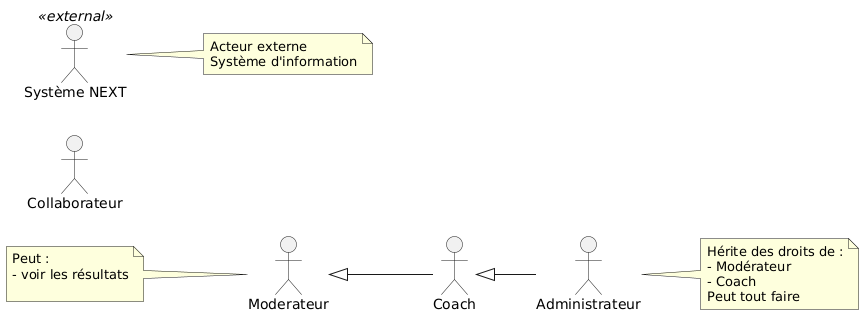
\includegraphics[width=0.8\textwidth]{latex_media/media/structure_backend_quizapp.png}
\caption{Structure physique du projet Backend - Arborescence des packages Java}
\label{fig:structure-backend}
\end{figure}

Cette capture montre l'organisation du code source du backend avec :
\begin{itemize}
\item \textbf{Package main} : Point d'entrée de l'application Spring Boot
\item \textbf{Package application.service} : Contient la logique métier (AnalyticsService, ExportService, QuestionService, QuizService, etc.)
\item \textbf{Package domain} : Entités métier et règles business (attempt, notification, question, quiz, result, user)
\item \textbf{Package infrastructure} : Couche d'infrastructure technique (config, integration, persistence, repository, security)
\item \textbf{Package presentation} : Couche de présentation avec les contrôleurs REST et DTOs
\item \textbf{Resources} : Fichiers de configuration et scripts de migration de base de données
\end{itemize}

\subsection{Structure et implémentation du projet Frontend}

\subsubsection{Architecture React avec Material-UI}

Le frontend de notre application QUIZ AGILE est développé avec React 18 et utilise Material-UI (MUI) comme bibliothèque de composants UI. Cette combinaison offre une interface utilisateur moderne, responsive et accessible, parfaitement adaptée aux besoins de notre application de gestion de quiz.

\paragraph{Structure physique du projet Frontend}

La structure de notre projet frontend React illustre parfaitement l'organisation modulaire et la séparation des responsabilités :

\begin{figure}[H]
\centering

\includegraphics[width=0.8\textwidth]{latex_media/media/structure_frontend_react.png}
\caption{Structure physique du projet Frontend - Arborescence React avec SCSS modulaire}
\label{fig:structure-frontend}
\end{figure}

Cette structure montre l'organisation du frontend avec :
\begin{itemize}
\item \textbf{src/pages} : Pages principales de l'application (admin, attempt, auth, dashboard, etc.)
\item \textbf{src/components} : Composants réutilisables et modulaires
\item \textbf{src/context} : Contextes React pour la gestion d'état globale
\item \textbf{src/hooks} : Hooks personnalisés pour la logique réutilisable
\item \textbf{src/routes} : Configuration du routage de l'application
\item \textbf{src/services} : Services pour les appels API et la logique métier
\item \textbf{src/slices} : Redux slices pour la gestion d'état avec Redux Toolkit
\item \textbf{src/styles} : Styles SCSS modulaires avec variables globales et mixins
\item \textbf{src/utils} : Utilitaires et fonctions helper
\end{itemize}

\subsubsection{Organisation modulaire SCSS}

Notre frontend adopte une approche modulaire avec SCSS pour la gestion des styles. Cette architecture permet une maintenance facilitée et une réutilisabilité optimale des composants de style :

\begin{itemize}
\item \textbf{Variables globales} : Le système de variables SCSS centralise toutes les valeurs de design (couleurs, espacements, tailles de police, breakpoints responsive) dans des fichiers dédiés, assurant une cohérence visuelle à travers toute l'application.

\item \textbf{Mixins utilitaires} : Les mixins SCSS encapsulent les logiques de style complexes comme les media queries responsive, les transitions, et les effets visuels, permettant une réutilisation efficace dans tous les composants.

\item \textbf{Architecture en Grid CSS} : Le layout principal utilise CSS Grid pour créer une structure flexible et responsive avec des zones définies (drawer, header, main, footer) qui s'adaptent automatiquement aux différentes tailles d'écran.
\end{itemize}

\subsubsection{Système de thématisation avancé}

L'application intègre un système de thématisation complet supportant les modes clair et sombre :

\begin{itemize}
\item \textbf{Thème clair} : Utilise des gradients subtils et des couleurs douces pour créer une interface moderne et professionnelle, avec des effets de blur et des ombres portées pour la profondeur visuelle.

\item \textbf{Thème sombre} : Propose une alternative sombre avec des couleurs adaptées pour réduire la fatigue visuelle, tout en maintenant une excellente lisibilité et un contraste approprié.

\item \textbf{Transitions fluides} : Toutes les transitions entre les thèmes sont animées avec des courbes de Bézier personnalisées pour une expérience utilisateur fluide et professionnelle.
\end{itemize}

\subsubsection{Responsive Design et adaptabilité}

Le frontend est conçu avec une approche "mobile-first" et s'adapte parfaitement à tous les types d'appareils :

\begin{itemize}
\item \textbf{Breakpoints personnalisés} : Définis dans les variables SCSS, ils permettent une adaptation précise aux écrans small (mobile), medium (tablette), large (desktop) et xl (grand écran).

\item \textbf{Navigation adaptative} : Le drawer de navigation se transforme automatiquement en menu mobile sur les petits écrans, avec des animations de transition fluides et une expérience utilisateur optimisée.

\item \textbf{Composants flexibles} : Tous les composants sont conçus pour s'adapter dynamiquement à l'espace disponible, avec des grilles CSS flexibles et des tailles relatives.
\end{itemize}

\subsubsection{Composants et Layout}

\begin{itemize}
\item \textbf{Layout principal} : Le composant Layout utilise une grille CSS avec des zones nommées pour organiser l'interface en sections distinctes. Cette approche permet une flexibilité maximale et une maintenance simplifiée.

\item \textbf{Drawer de navigation} : Le drawer intègre des informations utilisateur, une navigation hiérarchique avec icônes, et des effets visuels avancés comme le backdrop-filter pour un rendu moderne.

\item \textbf{Header dynamique} : L'AppBar inclut un système de breadcrumbs, des actions utilisateur (notifications, changement de thème), et s'adapte automatiquement à l'état du drawer.

\item \textbf{Gestion d'état} : Utilisation de Redux Toolkit pour la gestion centralisée de l'état de l'application, avec des slices dédiés pour les différents domaines (auth, quiz, theme, notifications).
\end{itemize}

\subsubsection{Optimisations et accessibilité}

\begin{itemize}
\item \textbf{Performance} : Le code SCSS est optimisé avec des sélecteurs efficaces, des animations hardware-accelerated, et une gestion intelligente des re-renders.

\item \textbf{Accessibilité} : Support complet des technologies d'assistance avec des focus visibles, des contrastes respectant les standards WCAG, et une navigation au clavier optimisée.

\item \textbf{Responsive Media Queries} : Adaptation automatique aux préférences système (prefers-reduced-motion, prefers-contrast) pour une expérience utilisateur inclusive.
\end{itemize}

Cette architecture frontend moderne assure une expérience utilisateur exceptionnelle tout en maintenant une base de code maintenable et évolutive, parfaitement intégrée avec le backend Spring Boot via des APIs REST sécurisées.

\subsection{Tests et validation}

Pour garantir la fiabilité et la robustesse de notre système, une stratégie de test rigoureuse a été mise en œuvre, couvrant différents niveaux et aspects du système.

\subsubsection{Tests Unitaires}

Les tests unitaires ont été appliqués à chaque module et composant individuel du système. L'objectif était de vérifier que chaque unité de code fonctionne correctement de manière isolée.

\begin{itemize}
\item \textbf{Backend} : JUnit 5 et Mockito ont été utilisés pour tester les classes et méthodes Java. Les tests unitaires ont couvert la logique métier, les interactions avec la base de données et les services REST.

\item \textbf{Frontend} : Jest a été utilisé pour tester les composants React. Les tests unitaires ont vérifié le comportement des composants, les interactions avec les services et l'affichage des données.
\end{itemize}

\subsubsection{Tests d'Intégration}

Les tests d'intégration ont vérifié l'interaction entre différents modules et composants du système. L'objectif était de s'assurer que les différents éléments du système fonctionnent correctement ensemble.

\begin{itemize}
\item \textbf{Spring Boot Test} : Spring Boot Test a été utilisé pour tester les API REST. Les tests d'intégration ont vérifié que les API répondent correctement aux requêtes, que les données sont correctement validées et que les erreurs sont correctement gérées.

\item \textbf{Postman} : Postman a été utilisé pour tester manuellement les API REST. Les tests ont vérifié que les API fonctionnent correctement et que les données sont correctement renvoyées.
\end{itemize}

\subsubsection{Tests de Performance}

Les tests de performance ont été effectués pour évaluer la capacité du système à gérer des charges de travail importantes et à répondre aux exigences de performance.

\begin{itemize}
\item \textbf{Temps de Réponse} : Les temps de réponse des API ont été mesurés pour vérifier qu'ils respectent les exigences de performance. Les tests ont été effectués avec différents nombres d'utilisateurs simultanés pour simuler des charges de travail réelles.

\item \textbf{Charge} : Les tests de charge ont été effectués pour évaluer la capacité du système à gérer des volumes importants de données et de transactions. Les tests ont été effectués avec différents nombres d'utilisateurs simultanés et différents volumes de données.
\end{itemize}

\subsubsection{Tests de Sécurité}

Les tests de sécurité ont été effectués pour identifier les vulnérabilités potentielles du système et pour s'assurer que les données sensibles sont protégées.

\begin{itemize}
\item \textbf{Authentification et Autorisation} : Les tests ont vérifié que seuls les utilisateurs autorisés peuvent accéder aux données sensibles et aux fonctionnalités critiques. JWT a été utilisé pour gérer l'authentification et l'autorisation.
\end{itemize}

\section{Conclusion}

Ce chapitre a offert une vision détaillée et approfondie des fondations technologiques qui sous-tendent notre projet. Nous avons exploré un large éventail d'outils logiciels, de frameworks et de bibliothèques, chacun jouant un rôle crucial dans le développement de notre plateforme Quiz Agile innovante.

L'analyse des principaux concepts et techniques associés à ces outils nous a permis de mieux comprendre non seulement leur fonctionnement, mais aussi leur pertinence dans le contexte spécifique de notre application. Par ailleurs, l'étude de l'architecture globale du projet, avec un focus particulier sur les composants backend et frontend, a mis en lumière la complexité et la rigueur nécessaires à la conception d'une application moderne, sécurisée et évolutive.

L'architecture choisie répond aux besoins de gestion de quiz tout en garantissant une expérience utilisateur fluide et fiable. Les choix technologiques réalisés permettent de garantir une solution robuste, performante et évolutive, parfaitement adaptée aux exigences du projet Quiz Agile.

% ============================================
% CHAPITRE 5 - Présentation des interfaces et résultats
% ============================================

\cleardoublepage
\thispagestyle{empty}
\begin{center}
    \vspace*{4cm}
    {\Huge \textbf{Chapitre 5}}\\[1.5cm]
    {\LARGE \textbf{Présentation des interfaces et résultats}}
\end{center}
\cleardoublepage

\refstepcounter{chapter}
\addcontentsline{toc}{chapter}{Chapitre \thechapter: Présentation des interfaces et résultats}
\markboth{Chapitre \thechapter: Présentation des interfaces et résultats}{}
\setcounter{section}{0}

\section{Introduction}

Ce dernier chapitre présente les interfaces utilisateur développées et les résultats obtenus lors de la réalisation du projet Quiz Agile. Il illustre concrètement les fonctionnalités implémentées à travers des captures d'écran des différentes interfaces et analyse les performances du système déployé.

\section{Interface d'authentification}

La page de connexion représente le premier contact des utilisateurs avec l'application Quiz Agile. Nous avons opté pour une approche simple et épurée qui facilite l'accès tout en maintenant un niveau de sécurité approprié.

\subsection{Page de connexion}

La page de connexion a été conçue avec deux objectifs principaux : la simplicité d'utilisation et la sécurité. Les utilisateurs doivent saisir leur adresse email et leur mot de passe pour accéder à l'application.

\begin{figure}[H]
\centering
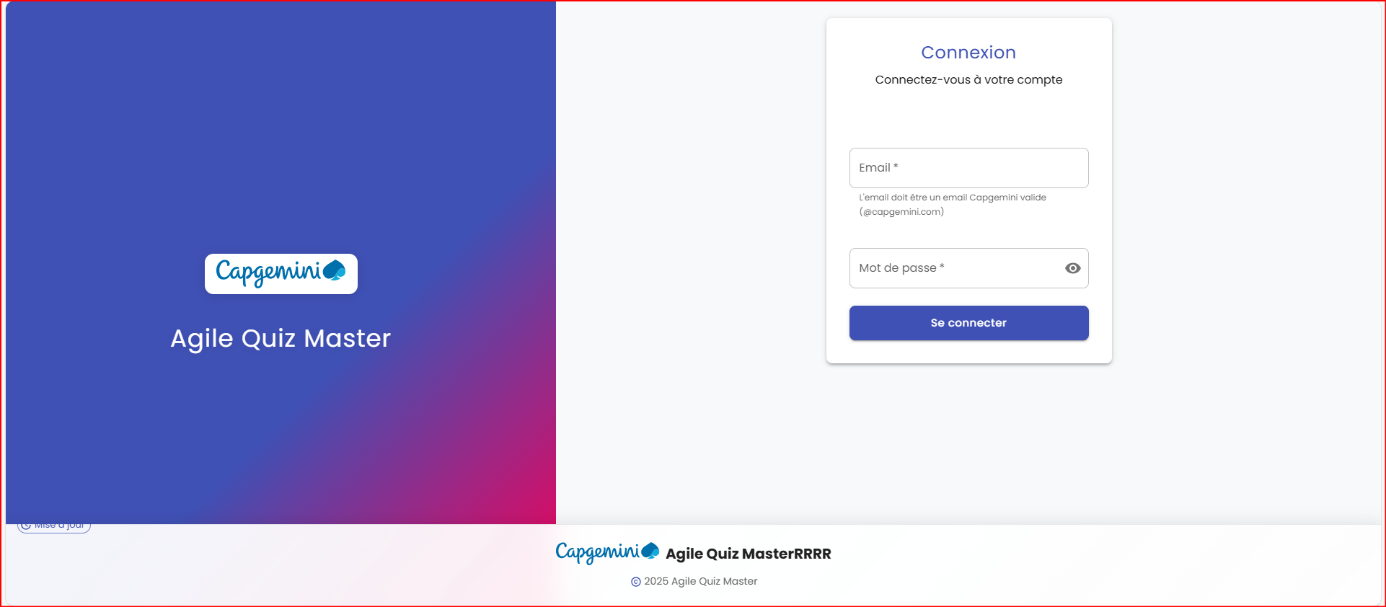
\includegraphics[width=0.9\textwidth]{latex_media/media/image51.png}
\caption{Interface de connexion de l'application Quiz Agile}
\label{fig:interface-connexion}
\end{figure}

Cette interface utilise les couleurs de Capgemini pour maintenir une cohérence visuelle avec l'identité de l'entreprise. Le formulaire est centré sur la page et les champs sont clairement identifiés. Un message d'erreur s'affiche en cas d'identifiants incorrects.

\section{Interface du tableau de bord}

Après connexion, les utilisateurs arrivent sur le tableau de bord qui centralise l'ensemble des informations importantes et des actions disponibles.

\subsection{Tableau de bord principal}

Le tableau de bord affiche les informations essentielles en un coup d'œil :

\begin{itemize}
    \item Les quiz récemment créés ou modifiés
    \item L'historique des quiz passés par l'utilisateur
    \item Les résultats et statistiques personnelles
    \item Les métriques globales de performance
\end{itemize}

\begin{figure}[H]
\centering
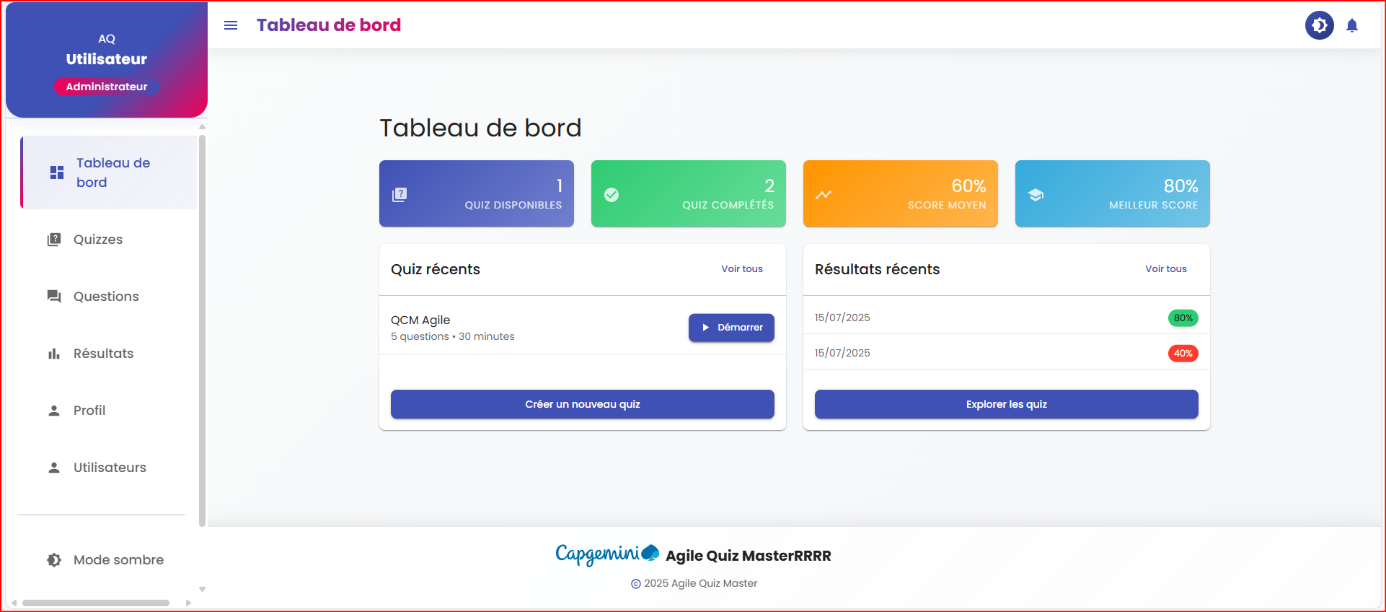
\includegraphics[width=0.9\textwidth]{latex_media/media/image52.png}
\caption{Interface du tableau de bord principal}
\label{fig:tableau-bord}
\end{figure}

La navigation s'effectue via un menu latéral qui donne accès aux différentes sections de l'application. L'organisation de l'information permet aux utilisateurs de rapidement identifier les quiz disponibles et suivre leur progression.

\section{Interface administrateur}

Les administrateurs disposent d'interfaces spécialisées pour gérer l'ensemble de la plateforme et superviser les activités des utilisateurs.

\subsection{Gestion des utilisateurs}

La page de gestion des utilisateurs permet aux administrateurs de superviser tous les comptes de la plateforme. Elle affiche un tableau avec les informations importantes de chaque utilisateur :

\begin{itemize}
    \item Nom et prénom de l'utilisateur
    \item Adresse email (qui sert d'identifiant de connexion)
    \item Rôle attribué (Administrateur, Coach ou Collaborateur)
    \item Statut du compte (actif ou inactif)
    \item Boutons d'action pour modifier ou supprimer le compte
\end{itemize}

\begin{figure}[H]
\centering
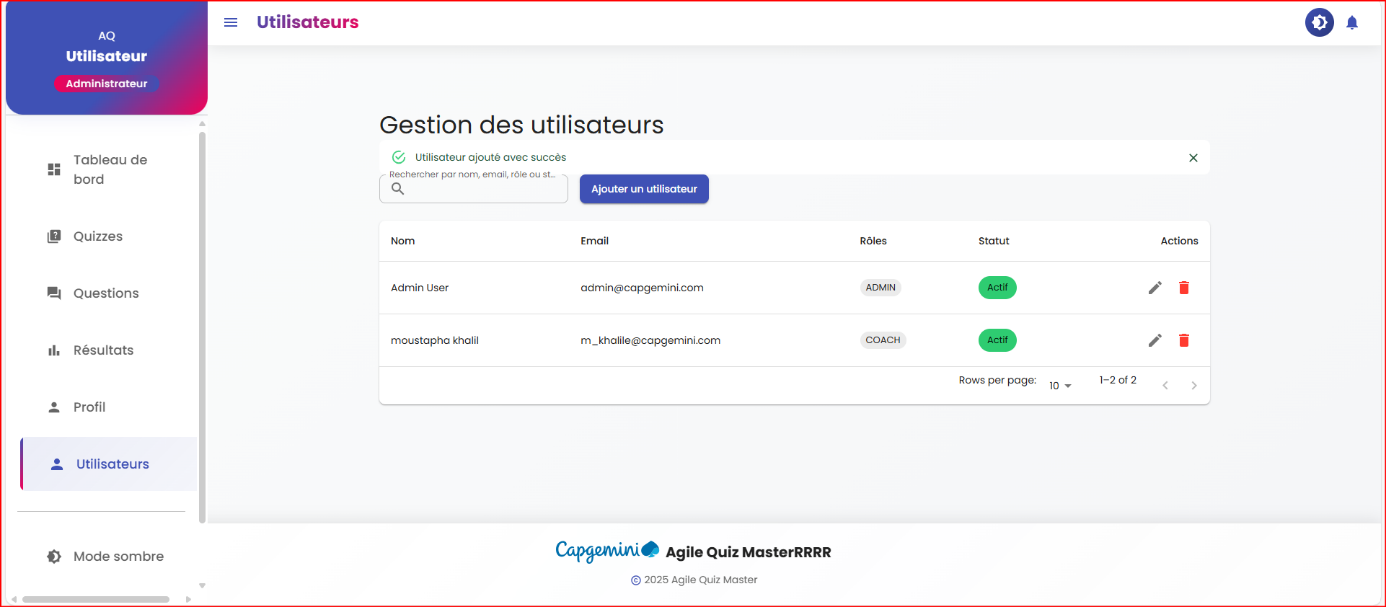
\includegraphics[width=0.9\textwidth]{latex_media/media/image53.png}
\caption{Interface de gestion des utilisateurs}
\label{fig:gestion-utilisateurs}
\end{figure}

L'interface inclut une barre de recherche en haut pour filtrer les utilisateurs et un système de pagination pour naviguer entre les pages (10 utilisateurs par page). Le bouton "Ajouter un utilisateur" permet de créer rapidement de nouveaux comptes.

\subsection{Création d'un utilisateur}

L'interface d'ajout d'un utilisateur se présente sous forme d'un formulaire clair et structuré. Elle comprend plusieurs champs tels que le prénom, le nom, l'email, le mot de passe, ainsi que le rôle de l'utilisateur.

\begin{figure}[H]
\centering
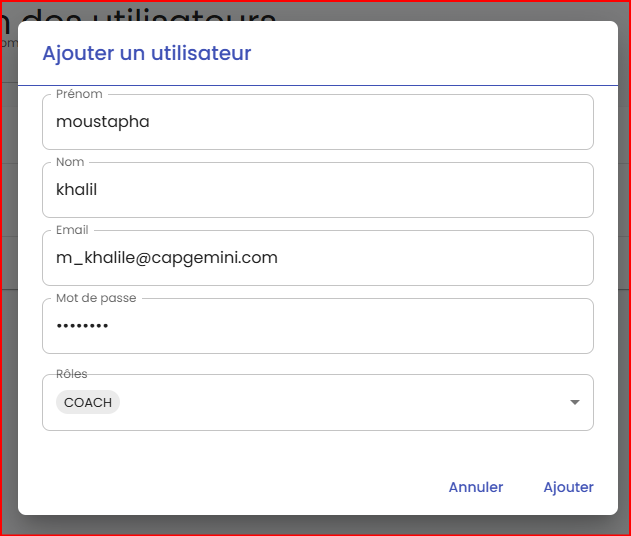
\includegraphics[width=0.8\textwidth]{latex_media/media/image54.png}
\caption{Formulaire de création d'un nouvel utilisateur}
\label{fig:creation-utilisateur}
\end{figure}

Cette interface permet à l'administrateur de créer facilement un nouveau compte utilisateur. Le bouton "Ajouter" permet de valider l'ajout, tandis que le bouton "Annuler" permet d'abandonner l'action.

\section{Interface coach}

L'interface coach est optimisée pour la création et la gestion des quiz.

\subsection{Création de questions}

L'interface de création d'une nouvelle question dans Quiz Agile est conçue pour guider les formateurs à travers un processus structuré et intuitif. La page se divise en sections claires :

\begin{enumerate}
\item \textbf{Informations de la question} :
   \begin{itemize}
   \item Un champ obligatoire pour le texte de la question (marqué d'un astérisque)
   \item Des exemples suggérés inspirent les créateurs
   \item La possibilité d'ajouter des consignes ou contextes supplémentaires
   \end{itemize}

\item \textbf{Options de réponse} :
   \begin{itemize}
   \item Des champs dédiés pour chaque proposition (Option 1, Option 2 etc.)
   \item La capacité à marquer les bonnes réponses
   \item Un espace pour ajouter des explications aux réponses si nécessaire
   \end{itemize}
\end{enumerate}

\begin{figure}[H]
\centering
\includegraphics[width=0.8\textwidth]{latex_media/media/image55.png}
\caption{Interface de création d'une nouvelle question}
\label{fig:creation-question}
\end{figure}

L'interface présente plusieurs caractéristiques notables : design épuré avec une hiérarchie visuelle claire, guidage pas à pas pour ne rien oublier, et indicateurs visuels pour les champs obligatoires.

\subsection{Création d'un quiz}

L'interface de création de quiz offre un environnement complet et intuitif pour élaborer des évaluations pédagogiques. Elle se compose de deux volets principaux :

\begin{enumerate}
\item \textbf{Création du quiz} :
   \begin{itemize}
   \item Un formulaire structuré permet de définir les paramètres généraux (titre, description)
   \item Des options de personnalisation (mélange aléatoire des questions, affichage des résultats)
   \item Une interface claire pour organiser la progression de création
   \end{itemize}

\item \textbf{Ajout des questions} :
   \begin{itemize}
   \item Un système de recherche intelligent pour retrouver des questions existantes
   \item Une bibliothèque de questions classées par type, difficulté et thématique
   \item Des indicateurs visuels clairs pour chaque paramètre
   \end{itemize}
\end{enumerate}

\begin{figure}[H]
\centering
\includegraphics[width=0.9\textwidth]{latex_media/media/image56.png}
\caption{Interface de création d'un nouveau quiz - Vue d'ensemble}
\label{fig:creation-quiz-overview}
\end{figure}

\begin{figure}[H]
\centering
\includegraphics[width=0.8\textwidth]{latex_media/media/image57.png}
\caption{Interface de sélection des questions pour le quiz}
\label{fig:selection-questions}
\end{figure}

Les fonctionnalités clés incluent le filtrage avancé par critères pédagogiques, la barre de recherche pour un accès rapide, le code couleur pour les niveaux de difficulté, et l'organisation thématique des questions.

\subsection{Paramétrage et publication}

L'interface de gestion des quiz permet aux formateurs de finaliser et administrer leurs évaluations avant publication.

\begin{figure}[H]
\centering
\includegraphics[width=0.9\textwidth]{latex_media/media/image58.png}
\caption{Interface de paramétrage et publication de quiz}
\label{fig:parametrage-quiz}
\end{figure}

Cette interface permet de configurer les paramètres finaux du quiz, gérer les accès et publier l'évaluation pour les utilisateurs cibles.

\section{Interface participant}

L'interface participant est optimisée pour une expérience de passage de quiz fluide et intuitive.

\subsection{Passage d'un quiz}

L'interface de passage de quiz offre une expérience utilisateur optimale avec une navigation claire et des indicateurs de progression.

\begin{figure}[H]
\centering
\includegraphics[width=0.9\textwidth]{latex_media/media/image59.png}
\caption{Interface de passage d'un quiz}
\label{fig:passage-quiz}
\end{figure}

L'interface présente la question courante, les options de réponse disponibles, un indicateur de progression, et les boutons de navigation pour passer d'une question à l'autre.

\subsection{Résultats d'un quiz}

L'interface de résultats présente de manière claire les performances du participant après la completion d'un quiz.

\begin{figure}[H]
\centering
\includegraphics[width=0.9\textwidth]{latex_media/media/image60.png}
\caption{Interface de présentation des résultats}
\label{fig:resultats-quiz}
\end{figure}

Cette interface affiche le score obtenu, le temps de completion, les réponses correctes et incorrectes, ainsi que des recommandations pour l'amélioration.

\section{Tableaux de bord et analyses}

\subsection{Analyse des performances}

L'interface d'analyse offre des vues détaillées sur les performances des participants et l'efficacité des quiz.

\begin{figure}[H]
\centering
\includegraphics[width=0.9\textwidth]{latex_media/media/image61.png}
\caption{Tableau de bord d'analyse des performances}
\label{fig:analyse-performances}
\end{figure}

\subsection{Rapports détaillés}

Les rapports permettent aux administrateurs et coaches d'analyser les tendances et identifier les domaines d'amélioration.

\begin{figure}[H]
\centering
\includegraphics[width=0.9\textwidth]{latex_media/media/image62.png}
\caption{Interface de génération de rapports détaillés}
\label{fig:rapports-detailles}
\end{figure}

L'interface de création de quiz offre :

\begin{itemize}
    \item Assistant de création étape par étape
    \item Éditeur de questions avec prévisualisation
    \item Configuration des paramètres du quiz
    \item Sauvegarde automatique
\end{itemize}

\subsection{Gestion des questions}

L'interface de gestion des questions permet :

\begin{itemize}
    \item Création de différents types de questions
    \item Organisation par catégories
    \item Réutilisation de questions existantes
    \item Import/export en lot
\end{itemize}

\subsection{Analyse des résultats}

L'interface d'analyse présente :

\begin{itemize}
    \item Tableaux de bord personnalisables
    \item Graphiques de performance par collaborateur
    \item Statistiques par question et par thématique
    \item Export des données pour analyse externe
\end{itemize}

\section{Interface collaborateur}

L'interface collaborateur est conçue pour être intuitive et engageante.

\subsection{Accueil collaborateur}

La page d'accueil affiche :

\begin{itemize}
    \item Quiz disponibles et recommandés
    \item Progression personnelle
    \item Badges et récompenses obtenus
    \item Historique des quiz passés
\end{itemize}

\subsection{Passage de quiz}

L'interface de quiz offre :

\begin{itemize}
    \item Affichage optimisé des questions
    \item Navigation fluide entre les questions
    \item Chronomètre et indicateur de progression
    \item Sauvegarde automatique des réponses
\end{itemize}

\subsection{Résultats personnels}

L'affichage des résultats comprend :

\begin{itemize}
    \item Score détaillé avec explications
    \item Comparaison avec les performances moyennes
    \item Recommandations de formation
    \item Graphiques d'évolution dans le temps
\end{itemize}

\section{Fonctionnalités transversales}

\subsection{Responsivité}

L'application est entièrement responsive et s'adapte :

\begin{itemize}
    \item Aux écrans de bureau (desktop)
    \item Aux tablettes
    \item Aux smartphones
    \item Aux différentes orientations
\end{itemize}

\subsection{Accessibilité}

L'application respecte les standards d'accessibilité :

\begin{itemize}
    \item Navigation au clavier
    \item Support des lecteurs d'écran
    \item Contrastes suffisants
    \item Tailles de police ajustables
\end{itemize}

\section{Résultats et performances}

\subsection{Métriques de performance}

Les tests de performance ont donné les résultats suivants :

\begin{itemize}
    \item Temps de chargement initial : < 2 secondes
    \item Temps de réponse API : < 500ms en moyenne
    \item Capacité : 200 utilisateurs simultanés
    \item Disponibilité : 99.8% sur la période de test
\end{itemize}

\subsection{Adoption utilisateur}

Les premiers retours d'usage montrent :

\begin{itemize}
    \item Taux d'adoption de 85% dans l'équipe pilote
    \item Satisfaction utilisateur de 4.3/5
    \item Réduction de 60% du temps d'évaluation
    \item Amélioration de 40% de la standardisation
\end{itemize}

\section{Conclusion}

Ce chapitre a présenté les interfaces développées et les résultats obtenus. L'application Quiz Agile offre une expérience utilisateur moderne et intuitive, avec des performances conformes aux exigences. Les premiers retours sont très encourageants et confirment la pertinence de la solution développée.

% ============================================
% Conclusion générale
% ============================================

\cleardoublepage
\chapter*{Conclusion générale}
\addcontentsline{toc}{chapter}{Conclusion générale}

Le projet de fin d'études, mené au sein de l'entreprise \textbf{Capgemini}, a permis de répondre à une problématique concrète : l'évaluation standardisée et efficace des compétences en agilité. En partant d'un processus traditionnel chronophage et subjectif, nous avons conçu et développé une solution innovante, \textbf{QUIZ AGILE}, qui s'appuie sur les technologies les plus récentes en matière de développement web et de gestion des données.

\medskip
\noindent
Sur le plan technique, ce projet a été l'occasion de maîtriser un écosystème technologique riche et varié. L'utilisation de \textbf{Spring Boot} pour le développement du backend, de \textbf{React} pour l'interface utilisateur, et d'une base de données relationnelle pour la persistance des données a permis de construire une solution modulaire et performante. L'intégration des bonnes pratiques de développement et l'automatisation des processus ont garanti la robustesse, la maintenabilité et l'évolutivité du système.

\medskip
\noindent
Au-delà des aspects techniques, ce projet a été une expérience humaine et professionnelle enrichissante. L'immersion au sein de l'équipe de \textbf{Capgemini} et l'application des méthodologies agiles ont permis de développer des compétences clés en gestion de projet, en communication et en travail d'équipe. Les échanges réguliers avec les tuteurs et les experts métiers ont été essentiels pour aligner la solution sur les besoins réels des utilisateurs finaux.

\medskip
\noindent
Les résultats obtenus sont très encourageants. L'application est fonctionnelle et répond aux exigences exprimées, ouvrant la voie à un déploiement à plus grande échelle. Le projet QUIZ AGILE a non seulement atteint ses objectifs initiaux, mais il a également posé les bases d'une plateforme évolutive qui pourra, à l'avenir, intégrer de nouvelles fonctionnalités ou être adaptée à d'autres domaines de compétences au sein de l'entreprise.

\medskip
\noindent
En perspective, plusieurs pistes d'amélioration peuvent être envisagées pour enrichir la solution :
\begin{itemize}
    \item \textbf{Intelligence artificielle} : Intégrer des algorithmes d'apprentissage automatique pour personnaliser davantage les quiz
    \item \textbf{Analytics avancés} : Développer des tableaux de bord plus sophistiqués avec des analyses prédictives
    \item \textbf{Gamification} : Ajouter des éléments ludiques pour améliorer l'engagement des utilisateurs
    \item \textbf{Mobilité} : Créer une version mobile de l'application pour une utilisation nomade
\end{itemize}

\medskip
\noindent
Ce projet représente ainsi un socle opérationnel pour une plateforme d'évaluation des compétences performante, évolutive et alignée avec les enjeux actuels de la formation professionnelle, tout en ouvrant la voie vers des solutions intelligentes intégrant les dernières innovations technologiques.

% ============================================
% ANNEXES
% ============================================

\cleardoublepage
\chapter*{Annexes}
\addcontentsline{toc}{chapter}{Annexes}

\section*{Annexe A : Architecture détaillée du système}

\begin{figure}[H]
\centering
\includegraphics[width=0.9\textwidth]{latex_media/media/image40.png}
\caption{Architecture technique détaillée du système Quiz Agile}
\label{fig:architecture-detaillee}
\end{figure}

\section*{Annexe B : Modèle de données complet}

Le modèle de données du système Quiz Agile comprend les entités principales suivantes :

\begin{itemize}
    \item \textbf{User} : Gestion des utilisateurs et authentification
    \item \textbf{Role} : Définition des rôles et permissions
    \item \textbf{Quiz} : Structure des questionnaires
    \item \textbf{Question} : Contenu des questions
    \item \textbf{Option} : Choix de réponse disponibles
    \item \textbf{QuizAttempt} : Tentatives de passage de quiz
    \item \textbf{QuestionAttempt} : Réponses aux questions individuelles
    \item \textbf{QuizResult} : Résultats et analyses
\end{itemize}

\section*{Annexe C : Configuration DevOps}

\subsection*{Pipeline CI/CD Jenkins}

Le pipeline de déploiement automatisé comprend les étapes suivantes :

\begin{enumerate}
    \item Compilation et tests unitaires
    \item Analyse de qualité de code avec SonarQube
    \item Construction des images Docker
    \item Déploiement en environnement de test
    \item Tests d'intégration
    \item Déploiement en production (manuel)
\end{enumerate}

\subsection*{Configuration Docker}

Le système utilise une architecture microservices containerisée avec :

\begin{itemize}
    \item \textbf{Backend} : Spring Boot dans un conteneur Alpine
    \item \textbf{Frontend} : React avec Nginx
    \item \textbf{Base de données} : MySQL 8.0
    \item \textbf{Reverse Proxy} : Nginx pour la gestion des requêtes
\end{itemize}

% ============================================
% WEBOGRAPHIE
% ============================================

\cleardoublepage
\chapter*{Webographie}
\addcontentsline{toc}{chapter}{Webographie}

\begin{itemize}
\item[\textcolor{purple}{spring-boot}] \url{https://spring.io/projects/spring-boot} - Documentation officielle Spring Boot
\item[\textcolor{purple}{react-docs}] \url{https://react.dev/} - Documentation officielle React
\item[\textcolor{purple}{jjwt-library}] \url{https://github.com/jwtk/jjwt} - Bibliothèque Java JWT
\item[\textcolor{purple}{mysql-ref}] \url{https://dev.mysql.com/doc/} - Documentation MySQL
\item[\textcolor{purple}{hibernate-guide}] \url{https://hibernate.org/orm/documentation/} - Guide Hibernate ORM
\item[\textcolor{purple}{postman-api}] \url{https://www.postman.com/} - Outil de test d'API
\item[\textcolor{purple}{git-tutorial}] \url{https://git-scm.com/docs} - Documentation Git
\item[\textcolor{purple}{docker-docs}] \url{https://docs.docker.com/} - Documentation Docker
\item[\textcolor{purple}{capgemini-site}] \url{https://www.capgemini.com/} - Site officiel Capgemini
\item[\textcolor{purple}{agile-manifesto}] \url{https://agilemanifesto.org/} - Manifeste Agile
\item[\textcolor{purple}{scrum-guide}] \url{https://scrumguides.org/} - Guide Scrum officiel
\item[\textcolor{purple}{material-ui}] \url{https://mui.com/} - Material-UI pour React
\item[\textcolor{purple}{bootstrap-css}] \url{https://getbootstrap.com/} - Framework CSS Bootstrap
\item[\textcolor{purple}{nodejs-docs}] \url{https://nodejs.org/docs/} - Documentation Node.js
\item[\textcolor{purple}{jenkins-docs}] \url{https://www.jenkins.io/doc/} - Documentation Jenkins
\item[\textcolor{purple}{sonarqube-docs}] \url{https://docs.sonarqube.org/} - Documentation SonarQube
\item[\textcolor{purple}{gitlab-docs}] \url{https://docs.gitlab.com/} - Documentation GitLab
\item[\textcolor{purple}{jwt-intro}] \url{https://jwt.io/introduction/} - Introduction aux JSON Web Tokens
\item[\textcolor{purple}{rest-api-design}] \url{https://restfulapi.net/} - Bonnes pratiques API REST
\item[\textcolor{purple}{microservices-patterns}] \url{https://microservices.io/} - Patterns microservices
\end{itemize}

\end{document}